\documentclass[12pt,a4paper]{article}
\usepackage[utf8]{inputenc}
\usepackage[spanish,english]{babel}
\usepackage{graphicx}
\usepackage[a4paper, total={17cm,25cm}]{geometry}
\usepackage{array}		% Para los sistemas de ecuaciones
\usepackage{amsmath}	% Para los entornos matemáticos
\usepackage{amssymb}	% Para la simbología matemática
\usepackage{float}
\usepackage{pgfplots}
\usepgfplotslibrary{external} 
\tikzexternalize
%\tikzset{external/force remake}

%%%%%%%%%%%%%%%%%%%%%%%%%%%%%%%%%%%%%%%%%%%%%%%%%%

\title{Desarrollo de un compilador para robots móviles}
\author{}
\date{}

%%%%%%%%%%%%%%%%%%%%%%%%%%%%%%%%%%%%%%%%%%%%%%%%%%

\begin{document}

\maketitle

	%%%%%%%%%%%%%%%%%%%%%%%%%%%%%%%%%%%%%%%%%%%%%%%%%%

	\begin{abstract}
    En el presente trabajo se describe el desarrollo de un compilador para el control de trayectorias de un robot móvil.
    El mismo genera como salida un código en MATLAB que permite simular la trayectoria que realizará, así como el código necesario para programar dicho robot.
	\end{abstract}
    
    %%%%%%%%%%%%%%%%%%%%%%%%%%%%%%%%%%%%%%%%%%%%%%%%%%
    
    \section{Introducción}
    Un compilador es el nexo que permite traducir el lenguaje de alto nivel, manejado por el programador, en un lenguaje de bajo nivel, que pueda interpretar el micro controlador que posea el robot.
    Además, debe tener los datos necesarios sobre el funcionamiento del robot objeto, que le permitan transformar las funciones del estilo "GIRAR( radio, tiempo )" en sus correspondientes tiempos e intensidades de activación de los diversos motores.
    
    En el presente desarrollo, el compilador bajo estudio también generará un código que permita simular la trayectoria que describirá el robot móvil, a fin de tener una primera aproximación previa a su puesta en práctica.
    
    Tanto el código que generará las instrucciones finales para el micro controlador como el necesario para la simulación de la trayectoria, serán desarrollados en MATLAB.
    
    %%%%%%%%%%%%%%%%%%%%%%%%%%%%%%%%%%%%%%%%%%%%%%%%%%
    
    \section{Compilador}
    Para llevar a cabo la conversión de instrucciones, el compilador deberá realizar un análisis previo a la generación del código de salida, en el cual corroborará que las instrucciones ingreasadas por el usuario sean correctas.
	\begin{figure}
	\centering
	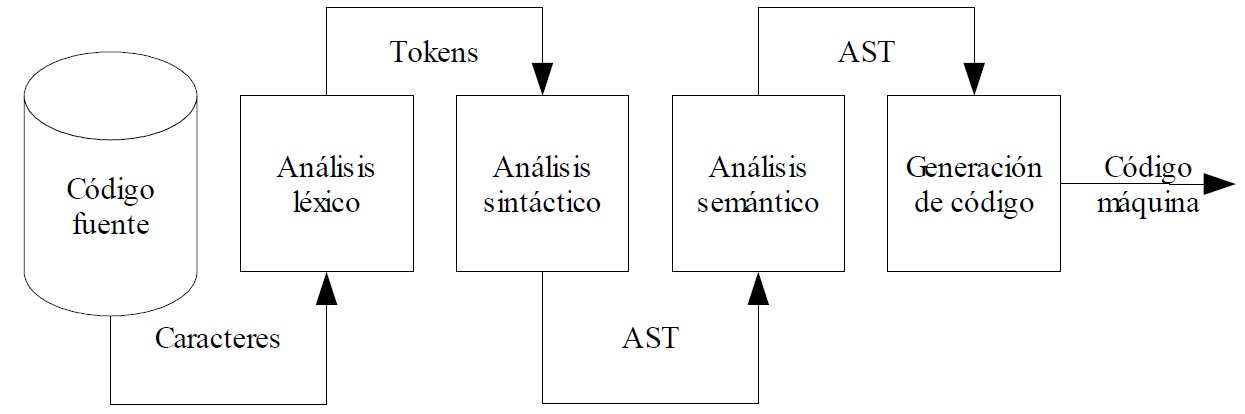
\includegraphics[width=0.7\linewidth]{./analisis}
    \caption{Etapas de un compilador}
    \label{etapas_del_compilador}
	\end{figure}
    Esto se puede esquematizar como la figura \ref{etapas_del_compilador}, donde se ve que se van realizando varios procesos en serie para realizar la compilación, como son:
    \begin{itemize}
		\item	Análisis léxico (Scanner): Como punto de partida, se convierte el código fuente en una serie de Tokens, que son símbolos léxicos definidos para el lenguaje, pudiendo ser\\
        		asimilados la idea de las palabras de una lengua.
        		Se reconocen las palabras reservadas del lenguaje y se verifican los tipos de datos utilizados
                
		\item	Análisis sintáctico (Parser): Se agrupan los tokens reconocidos en frases gramaticales para ser procesados mediante las reglas sintácticas, como la indicada en la figura \ref{Sintaxis}.
        		Se debe analizar la secuencia de tokens y datos asociados a cada instrucción válida.
                Aquí se tiene la representación de los diferentes estructuras de árbol AST (Abstract Syntax Tree) del programa, los cuales son una representación gráfica muy útil para la comprensión de lo descripto anteriormente, como se observa en la figura \ref{AST}.
                
		\item	Generación del código final: Verificada la sintaxis, se realiza la conversión de instrucciones.

	\end{itemize}
    
    \begin{figure}[!h]
    \centering
        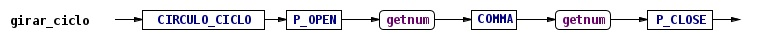
\includegraphics[width=0.7\linewidth]{./Rule_Ciclo.jpg}
    	\caption{Regla de sintáxis ejemplo para una instrucción}
    	\label{Sintaxis}
    \end{figure}
    
    \begin{figure}[!h]
    \centering
        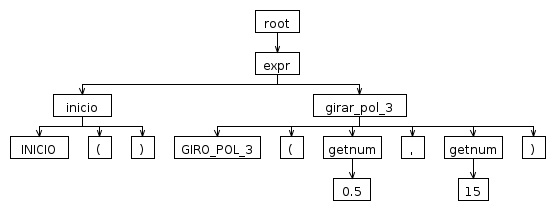
\includegraphics[width=0.7\linewidth]{./AST_ejemplo.jpg}
    	\caption{Árbol AST para las primeras 2 instrucciones}
    	\label{AST}
    \end{figure}
    
    El compilador se desarrolló en base al IDE ANTLRWorks 1.4.2, el cual permite realizar los análisis antes mencionados, simplificando el trabajo requerido, a la vez que tiene diversas herramientas gráficas para la representación de los diferentes flujos de tokens y demás.
    
    El robot empleado como target del compilador es el Multiplo N6.
    Este es un robot del tipo diferencial con una rueda libre en la parte posterior para mejorar su estabilidad, como se observa en la figura \ref{N6}
    
	\begin{figure}[h]
	\centering
	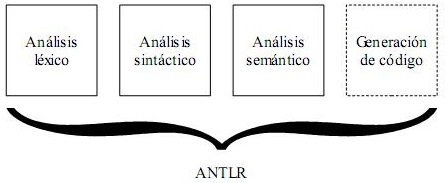
\includegraphics[width=0.7\linewidth]{./antlr.jpg}
    \caption{Herramientas del IDE ANTLRWorks 1.4.2}
	\end{figure}
    
	\begin{figure}
	\centering
	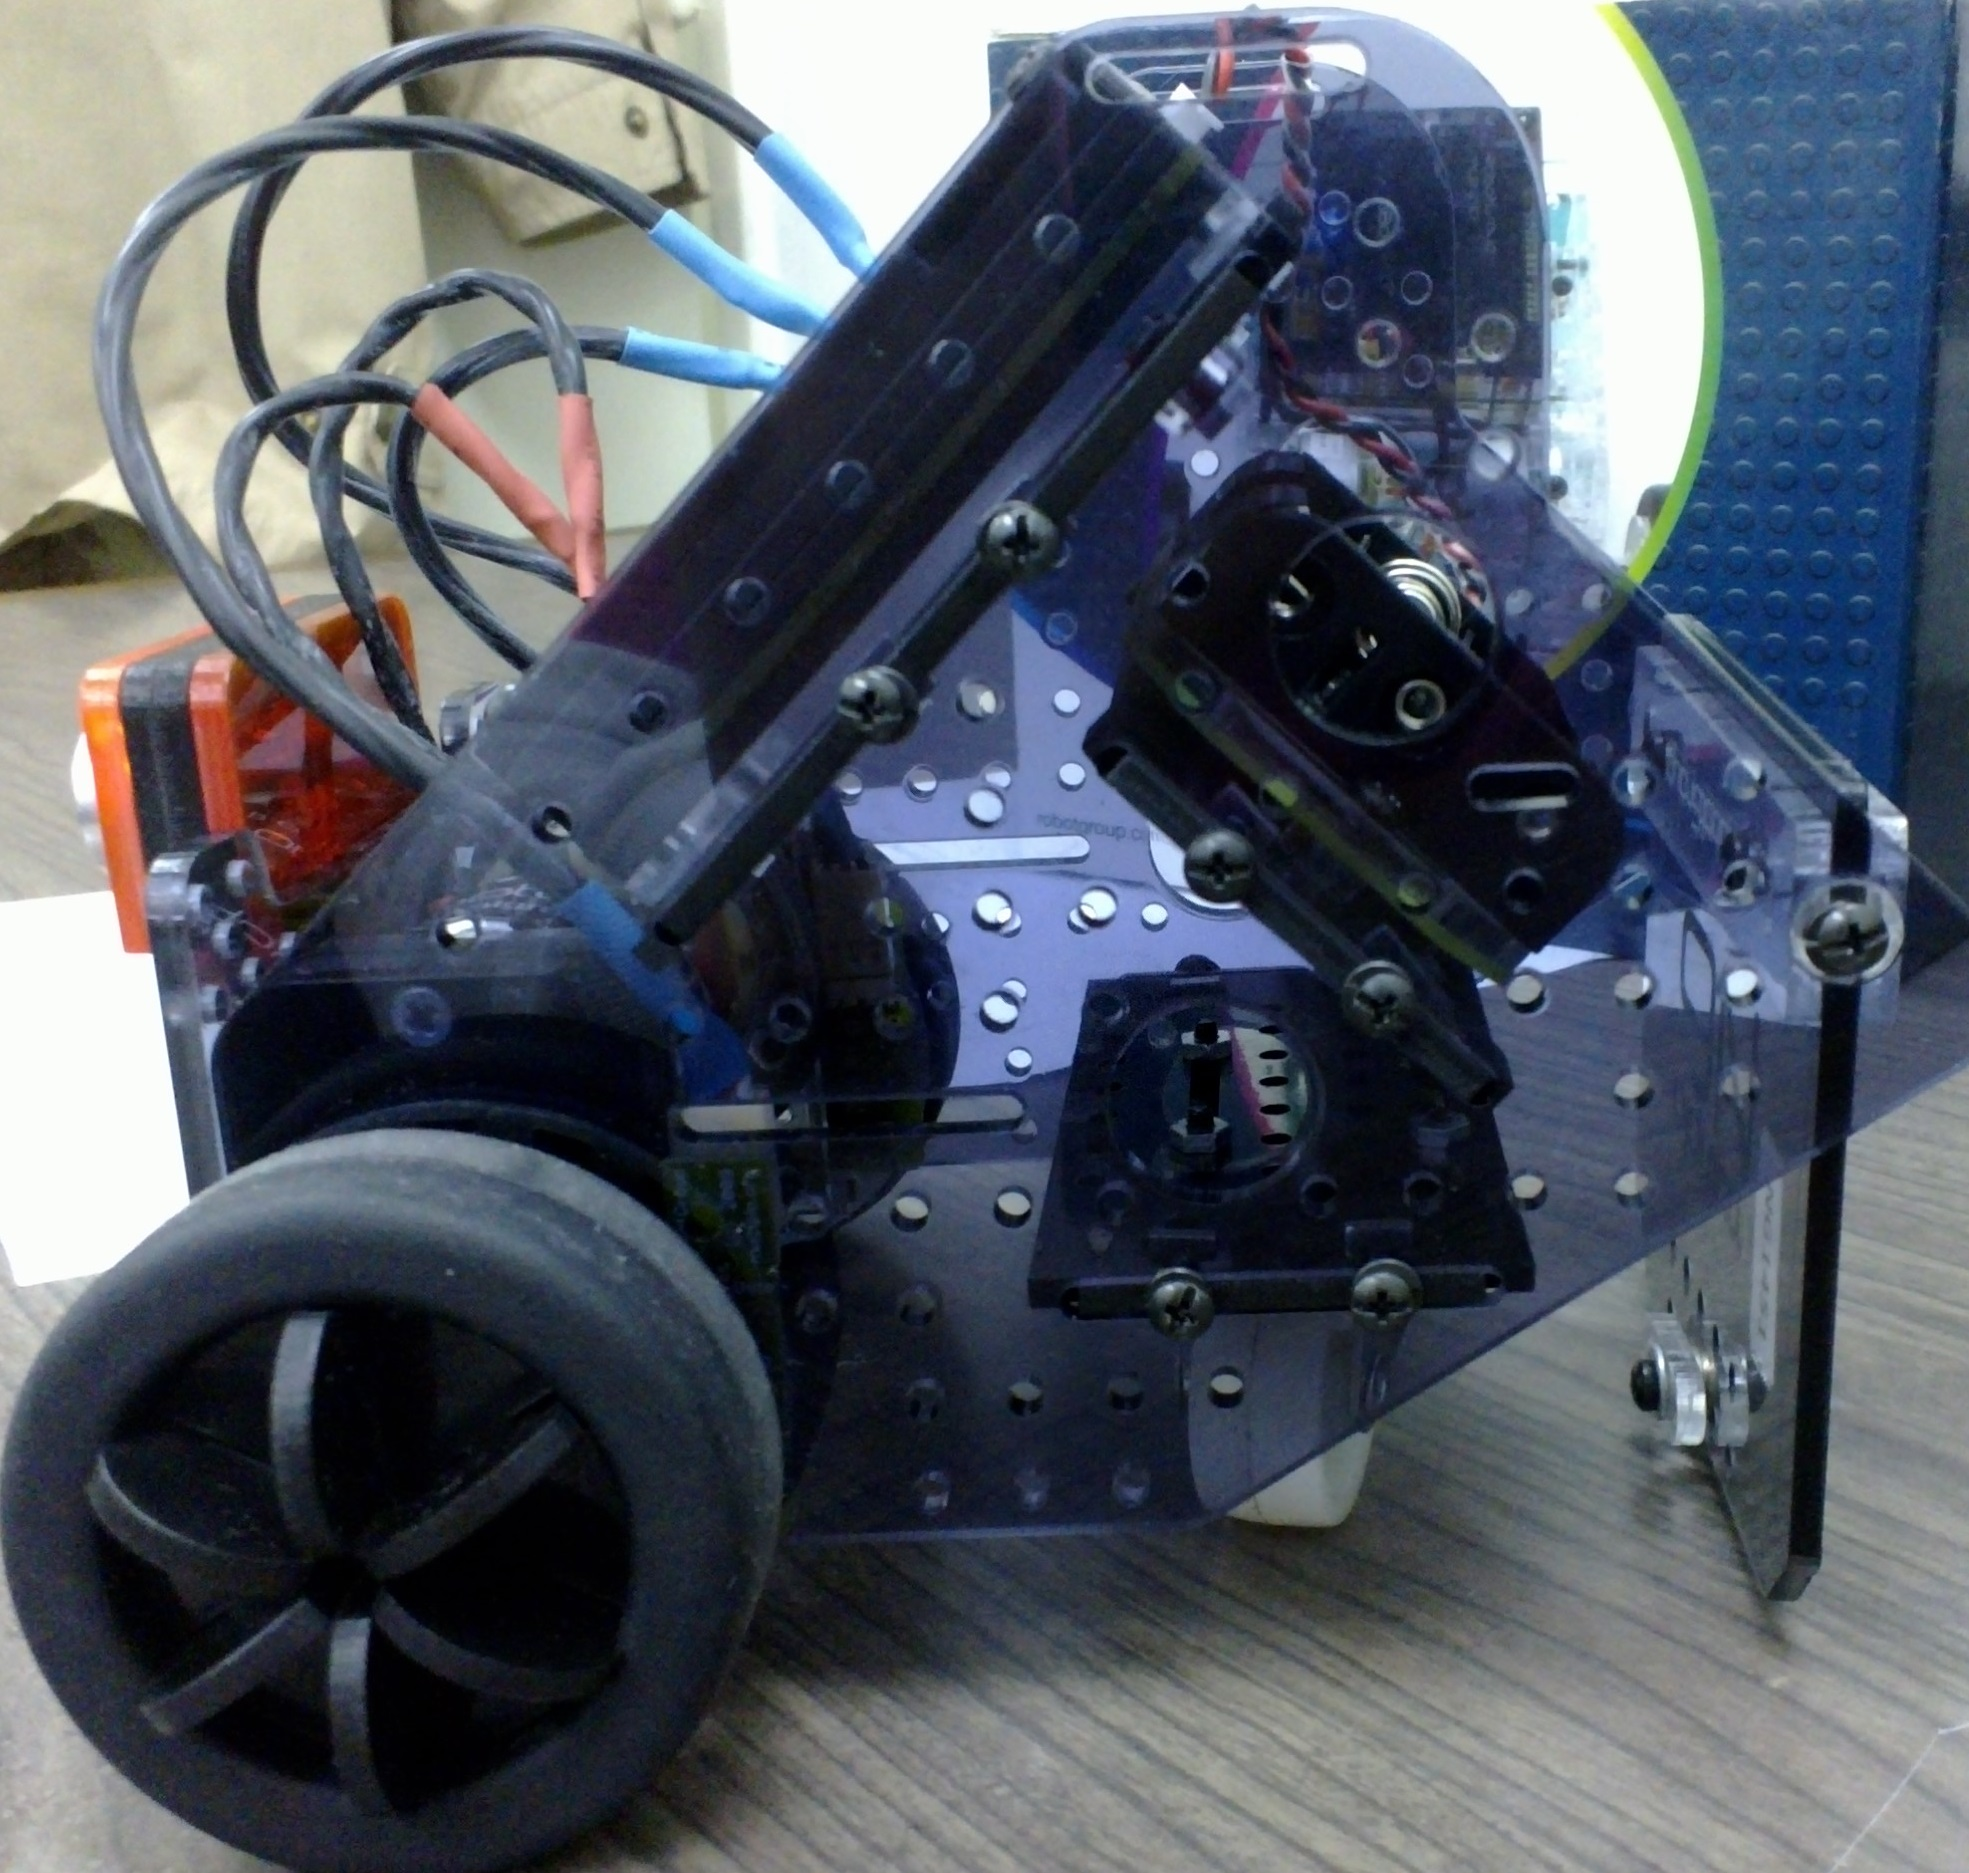
\includegraphics[width=0.4\linewidth]{./N6}
    \caption{Robot empleado como target}
    \label{N6}
	\end{figure}
    
	%%%%%%%%%%%%%%%%%%%%%%%%%%%%%%%%%%%%%%%%%%%%%%%%%%
    
    \section{Análisis cinemático}
    
    En el campo de la robótica movil se requiere desarrollar un modelo cinemático fiel del robot, ya que cuando este deba realizar una tarea, deberá reconocer en cada instante, mediante diversos sensores, el entorno que lo rodea.
    En función de su concepcion del ambiente y su modelo, deberá decidir en tiempo real que acciones tomar para su desplazamiento.
    
    A diferencia de los actuadores, los robots móviles no disponen de una referencia fija anclada a una estructura que les permita tener un punto de referencia absoluto sobre el cual basar sus decisiones, sino que se deben tomar siempre referencias relativas a un punto de partida o un punto anterior.
    Por esto, al existir algun error en el calculo del desplazamiento, se obtendrá una imperfección en el punto al cual se quiera arribar, el cual se sumara en cada movimiento, pudiendo ocasionar que el resultado final no sea el previsto.
    Por lo tanto, cuanto más exacto sea el modelo cinemático del robot móvil, sera posible seguir más fehacientemente la premisa de una trayectoria, desviándose lo menos posible del punto final.
    
	Según la teoría de cinemática directa desarrollada por Dudek \& Jenkin, para un robot con manejo diferencial, el par de ruedas esta montado sobre un eje común.
    Además, se pueden realizar las siguientes suposiciones:
    \begin{itemize}
		\item	El robot se mueve sobre una superficie plana sin irregularidades ni defectos del suelo.
        \item	Los ejes de guiado son perpendiculares al suelo.
        \item	Las ruedas se mueven con rodadura pura, es decir, el deslizamiento es despreciable.
	\end{itemize}
    
	De esta forma, si las ruedas del robot giran sobre el suelo con diferentes velocidades, entonces habrá un punto, denominado $ICC$ (Centro Instántaneo de Curvatura), alrededor del cual ambas giran y describen una trayectoria circular.
    Las ecuaciones para determinar la ubicación del punto de giro y la velocidad con que se desplaza el robot, son las siguientes:
    
    \begin{align}
		R = \dfrac{l}{2} \cdot \dfrac{ v_r + v_l }{ v_r - v_l }\\[0.3cm]
        \omega = \dfrac{ v_r - v_l }{ l }
	\end{align}
    
	%%%%%%%%%%%%%%%%%%%%%%%%%%%%%%%%%%%%%%%%%%%%%%%%%%
    
    \section{Análisis dinámico}
    
    El estudio del modelo dinámico de un robot permite obtener el torque que se le debe aplicar a cada articulación, tal que dicho mecanismo alcance las aceleraciones necesarias para realizar una determinada trayectoria.
    Ademas, en función del tipo de interpolador que se emplee para diseñar la trayectoria requerida, variará tanto la forma como los valores máximos, RMS y la continuidad o no de las curvas de velocidad y aceleración necesarias.
    Teniendo en cuenta la aplicacion que deba llevar a cabo el robot, se podrá limitar el uso de algún interpolador según se necesitase que la aceleración no presente discontinuidades, que su valor RMS o que su relación con el máximo sea la mínima posible, etc.
    
	El modelo dinámico se plantea mediante el uso de la mecanica de Lagrange, basado en consideraciones energéticas, segén el cual se deben definir las siguientes ecuaciones:
    
    \begin{align}
		\frac{\partial}{\partial x}\frac{\partial L}{\partial \dot{q}_i}-\frac{\partial L}{\partial q_i}=\tau \\[0.2cm]
        L=k-u
	\end{align}
    
    Donde:

    \begin{itemize}
    	\item	$q_i$: Coordenadas generalizadas.
    	\item	$\tau$: Vector de fuerzas y pares aplicados en las $q_i$.
    	\item	$L$: Función Lagrangiana.
    	\item	$k$: Energía cinética.
	    \item	$u$: Energía potencial.
    \end{itemize}
    
    En el caso de una aplicación donde el robot se moverá siempre sobre una superficie a la misma altura, se puede considerar que la energía potencial es nula, con lo cual el lagrangiano sólo está compuesto de las energías cinéticas correspondientes a:

    \begin{itemize}
    	\item	$K_1$: Energía cinética de traslación del robot completo
    	\item	$K_2$: Energía cinética de rotación del robot completo	
    	\item	$K_3$: Energía cinética de rotación del conjunto motor – rueda
    \end{itemize}

	\begin{align}
		K_1 =\frac{1}{2}m\left(x_c^2+y_c^2\right)\\[0.2cm]
        K_2 =\frac{1}{2}I_A\dot{\Theta}^2\\[0.2cm]
        K_3 =\frac{1}{2}I_0\dot{\Theta}^2_L+\frac{1}{2}I_0\dot{\Theta}^2_R
	\end{align}

	Donde $I_A$ es el momento de inercia del robot respecto al centro de masa, $I_0$ es el momento de inercia del conjunto motor--rueda respecto al centro de rotación.
    Los parámetros físicos del robot se obtienen mediante el desarrollo del modelo en el software Solidwroks mostrado en la figura \ref{N6_Solid}.
    
    \begin{figure}[!h]
    \centering
    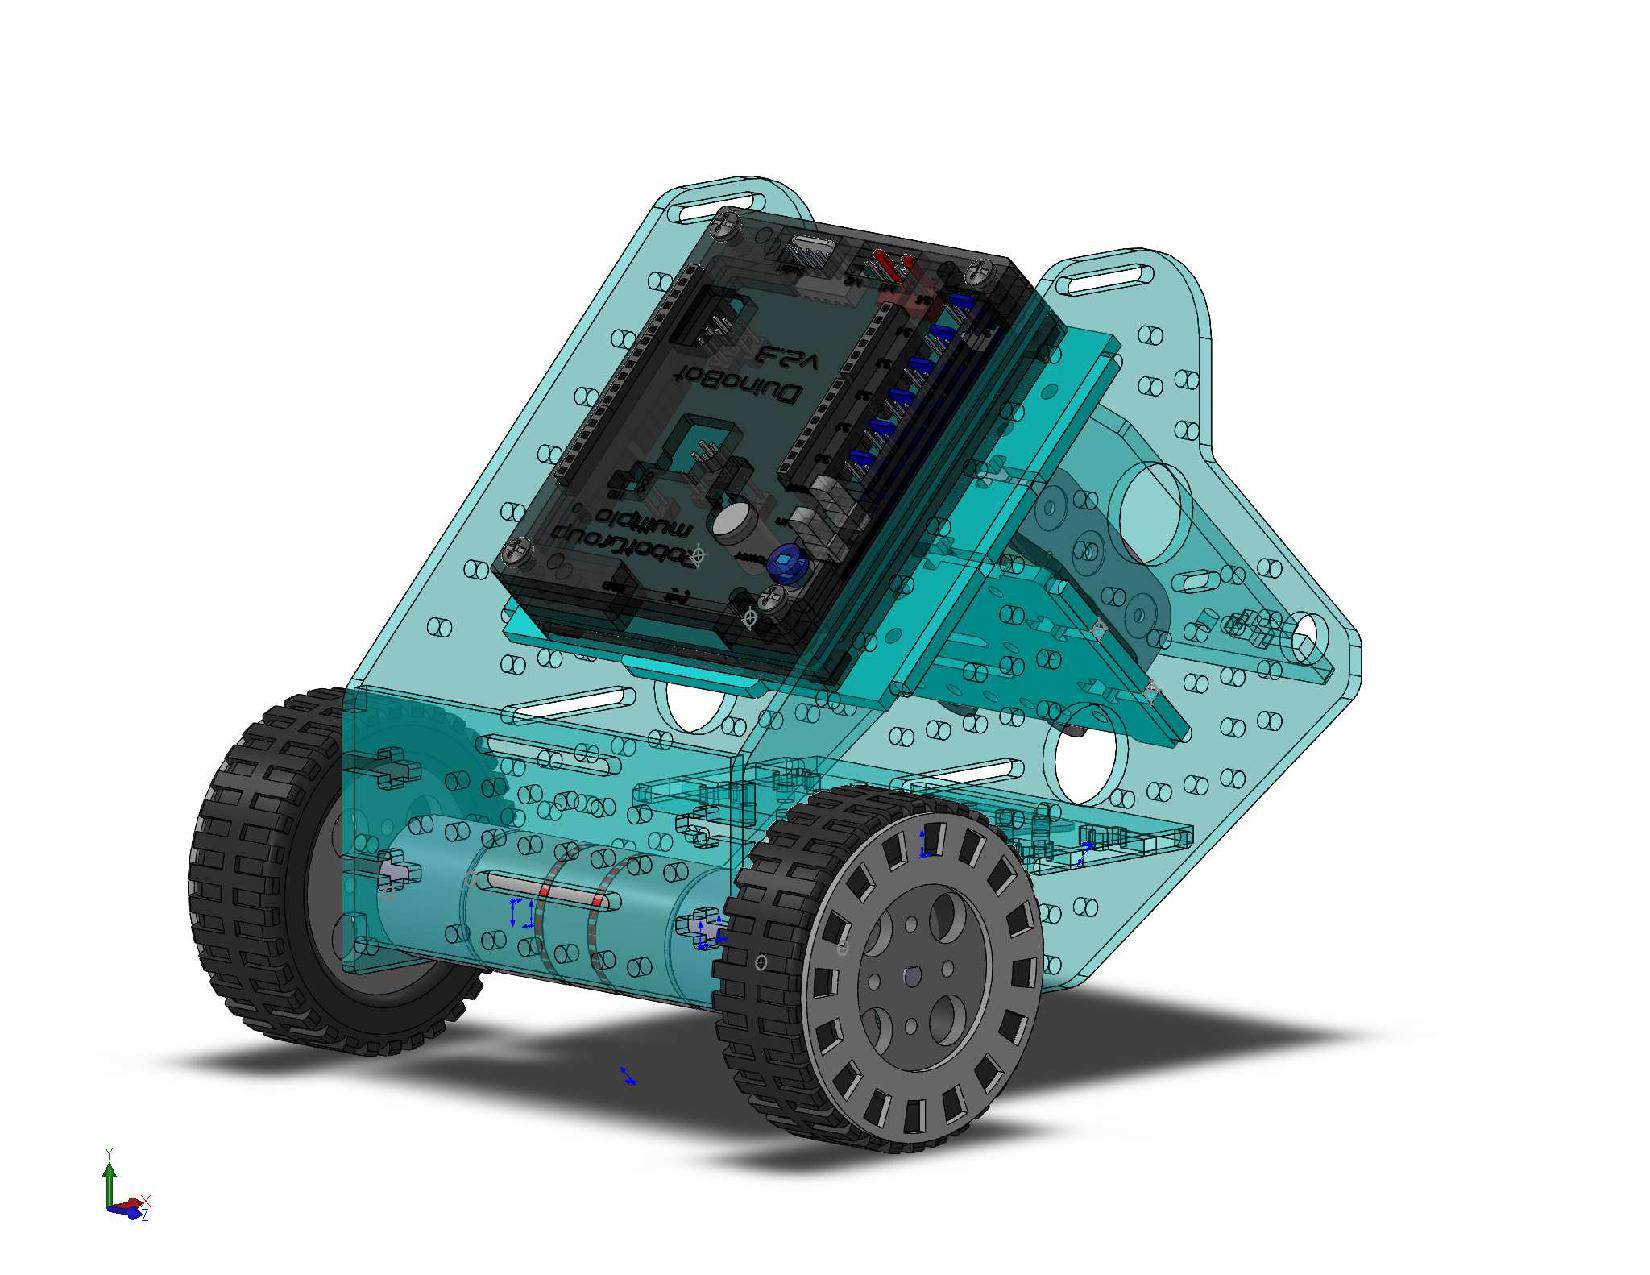
\includegraphics[width=0.5\linewidth]{./N6_Solid}
    \caption{Modelo del robot en Solidworks.}
    \label{N6_Solid}
    \end{figure}
    
	%%%%%%%%%%%%%%%%%%%%%%%%%%%%%%%%%%%%%%%%%%%%%%%%%%
    
    \section{Set de instrucciones propuesto}
    
    Como lenguaje de alto nivel para el usuario, se propone el siguiente set de instrucciones:
    
    \begin{itemize}
		\item[]	\verb|INICIO( modelo de robot )|:\\
        		Se encarga de inicializar el robot en cuestión.
        
        \item[]	\verb|GIRO_POL_3( radio, segundos )|:\\
        		Realiza un giro completo del radio indicado en la cantidad de segundos exigida, empleando el interpolador polinomial de orden 3:
                
        \item[]	\verb|GIRO_POL_5( radio, segundos )|:\\
        		Realiza un giro completo del radio indicado en la cantidad de segundos exigida, empleando el interpolador polinomial de orden 5:
                
        \item[]	\verb|GIRO_CICLO( radio, segundos )|:\\
        		Realiza un giro completo del radio indicado en la cantidad de segundos exigida, empleando el interpolador cicloidal:
                
		\item[]	\verb|GRAFICAR_VELOCIDADES()|:\\
        		Muestra el gráfico de las velocidades que desarrollarán las ruedas del robot.
                
		\item[]	\verb|GRAFICAR_TRAYECTORIA()|:\\
        		Muestra el gráfico de la trayectoria descrita por el robot.
                
		\item[]	\verb|EXPORTAR()|:\\
        		Genera el archivo necesario para programar el robot en cuestión con la trayectoria diseñada hasta esta instrucción.
        
	\end{itemize}
    
    %%%%%%%%%%%%%%%%%%%%%%%%%%%%%%%%%%%%%%%%%%%%%%%%%%
    
    \section{Ejemplo de uso}
    
    La siguiente rutina permite iniciar al robot, realizar 3 giros con distintos parámetros y mediante los diferentes interpoladores, obtener una gráfica de las velocidades de las ruedas y de la trayectoria esperada, y generar el código necesario para programar al robot target para desarrollar dicha trayectoria.
    
    \begin{verbatim}
    INICIO(N6)
    GIRO_POL_3(0.5,15)
    GIRO_POL_5(0.1,4)
    GIRO_CICLO(0.3,10)
    GRAFICAR_VELOCIDADES()
    GRAFICAR_TRAYECTORIA()
    EXPORTAR()
	\end{verbatim}
    
    \begin{figure}[H]
    \centering
    % This file was created by matlab2tikz.
%
%The latest updates can be retrieved from
%  http://www.mathworks.com/matlabcentral/fileexchange/22022-matlab2tikz-matlab2tikz
%where you can also make suggestions and rate matlab2tikz.
%
\definecolor{mycolor1}{rgb}{1.00000,0.00000,1.00000}%
%
\begin{tikzpicture}[trim axis left, trim axis right]

\begin{axis}[%
width=4.521in,
height=4.521in,
at={(0.758in,0.481in)},
scale only axis,
separate axis lines,
every outer x axis line/.append style={black},
every x tick label/.append style={font=\color{black},/pgf/number format/fixed},
xmin=-0.2,
xmax=0.2,
xlabel={Meters},
xmajorgrids,
every outer y axis line/.append style={black},
every y tick label/.append style={font=\color{black},/pgf/number format/fixed},
ymin=-0.2,
ymax=0.2,
ylabel={Meters},
ymajorgrids,
axis background/.style={fill=white},
]
\addplot [color=black,only marks,mark=x,mark options={solid},forget plot]
  table[row sep=crcr]{%
0.15	0\\
0.149988156630572	0.00188490598250289\\
0.149893420896088	0.00565352740049018\\
0.149573835039092	0.0112990208291899\\
0.148817205197172	0.0187999850346456\\
0.147343087609303	0.0281071971878587\\
0.144807245824991	0.0391262259434845\\
0.140810078648081	0.0516964384761775\\
0.134910787734956	0.0655673649976399\\
0.126649188825302	0.0803740192468495\\
0.115576986416368	0.0956135984623034\\
0.101299921218154	0.110626967603726\\
0.0835313424732281	0.124589384879372\\
0.0621563371489925	0.136515895602749\\
0.0373034830747281	0.145287474169295\\
0.00941857792939688	0.149704009264241\\
-0.0206685436026958	0.148569213854498\\
-0.0516964384761777	0.140810078648081\\
-0.0819591520101405	0.125629206006321\\
-0.109345294113212	0.102682065889303\\
-0.13144600200658	0.0722630511152572\\
-0.145744759937201	0.0354748495535586\\
-0.149893420896088	-0.00565352740049031\\
-0.142064745749212	-0.0481415414710815\\
-0.121352549156242	-0.0881677878438711\\
-0.088167787843871	-0.121352549156242\\
-0.0445562372365553	-0.143229681711997\\
0.00565352740049011	-0.149893420896089\\
0.0569668643282701	-0.138761581025169\\
0.102682065889303	-0.109345294113212\\
0.135724057869903	-0.0638668937347611\\
0.149810543490903	-0.00753664772696559\\
0.140810078648081	0.0516964384761774\\
0.108046353733186	0.104047995871921\\
0.0552186829027014	0.139466472883237\\
-0.00941857792939727	0.14970400926424\\
-0.073909101232244	0.130527563200428\\
-0.124589384879372	0.0835313424732277\\
-0.149041696578001	0.0169284577310217\\
-0.139466472883238	-0.0552186829027022\\
-0.0956135984623034	-0.115576986416369\\
-0.0262534588462913	-0.147684650179381\\
0.0516964384761776	-0.140810078648081\\
0.116769345235053	-0.0941537041936051\\
0.148817205197171	-0.0187999850346456\\
0.135724057869902	0.0638668937347609\\
0.0787761944941938	0.127649172269204\\
-0.0056535274004908	0.149893420896088\\
-0.0896857474586284	0.120235047730631\\
-0.142658477444273	0.0463525491562415\\
-0.142658477444273	-0.0463525491562427\\
-0.0866359055133401	-0.122450887607578\\
0.00565352740049033	-0.149893420896089\\
0.0970583942354168	-0.114366376651717\\
0.147343087609303	-0.0281071971878588\\
0.131446002006579	0.0722630511152571\\
0.0534617818069872	0.140149341368492\\
-0.0516964384761779	0.140810078648081\\
-0.132343683965243	0.0706055898247994\\
-0.145287474169295	-0.0373034830747287\\
-0.0803740192468491	-0.126649188825303\\
0.0299564970771614	-0.146978257857637\\
0.124589384879372	-0.0835313424732282\\
0.146978257857637	0.0299564970771611\\
0.0803740192468494	0.126649188825302\\
-0.0373034830747284	0.145287474169294\\
-0.132343683965243	0.0706055898247994\\
-0.140810078648081	-0.051696438476178\\
-0.0534617818069871	-0.140149341368492\\
0.0722630511152578	-0.131446002006579\\
0.147343087609303	-0.0281071971878582\\
0.114366376651717	0.097058394235417\\
-0.00565352740049099	0.149893420896088\\
-0.122450887607578	0.0866359055133389\\
-0.142658477444273	-0.0463525491562435\\
-0.046352549156241	-0.142658477444274\\
0.0896857474586288	-0.120235047730632\\
0.149893420896089	0.00565352740048995\\
0.0787761944941954	0.127649172269204\\
-0.0638668937347598	0.135724057869903\\
-0.14881720519717	0.0187999850346452\\
-0.094153704193603	-0.116769345235054\\
0.0516964384761797	-0.140810078648081\\
0.147684650179382	-0.0262534588462905\\
0.0956135984623045	0.115576986416369\\
-0.0552186829027007	0.139466472883238\\
-0.149041696578	0.0169284577310227\\
-0.0835313424732279	-0.124589384879372\\
0.073909101232244	-0.130527563200429\\
0.149704009264241	0.00941857792939722\\
0.0552186829027014	0.139466472883238\\
-0.104047995871921	0.108046353733185\\
-0.140810078648081	-0.0516964384761783\\
-0.00753664772696475	-0.149810543490903\\
0.135724057869904	-0.0638668937347612\\
0.109345294113213	0.102682065889303\\
-0.0569668643282691	0.138761581025169\\
-0.149893420896088	-0.00565352740048949\\
-0.0445562372365543	-0.143229681711996\\
0.121352549156243	-0.0881677878438699\\
0.121352549156242	0.0881677878438721\\
-0.0481415414710817	0.142064745749211\\
-0.149893420896087	-0.0056535274004917\\
-0.0354748495535555	-0.145744759937201\\
0.131446002006582	-0.0722630511152551\\
0.102682065889303	0.109345294113213\\
-0.0819591520101412	0.125629206006321\\
-0.140810078648079	-0.0516964384761789\\
0.0206685436026983	-0.148569213854498\\
0.149704009264242	-0.0094185779293956\\
0.0373034830747268	0.145287474169294\\
-0.136515895602749	0.0621563371489893\\
-0.0835313424732242	-0.124589384879374\\
0.11062696760373	-0.101299921218152\\
0.115576986416367	0.0956135984623052\\
-0.0803740192468511	0.1266491888253\\
-0.134910787734953	-0.0655673649976432\\
0.0516964384761814	-0.140810078648081\\
0.144807245824992	0.0391262259434859\\
-0.0281071971878591	0.147343087609303\\
-0.14881720519717	-0.0187999850346471\\
0.0112990208291931	-0.149573835039091\\
0.14989342089609	0.00565352740049296\\
-0.00188490598250418	0.149988156630573\\
-0.149999999999999	-1.73038666728687e-15\\
3.03704771181041e-15	-0.149999999999999\\
0.149988156630574	0.00188490598250505\\
-0.00565352740049035	0.149893420896089\\
-0.149573835039092	-0.0112990208291901\\
0.0187999850346467	-0.148817205197171\\
0.147343087609303	0.0281071971878603\\
-0.039126225943486	0.144807245824991\\
-0.14081007864808	-0.0516964384761785\\
0.0655673649976414	-0.134910787734955\\
0.126649188825302	0.0803740192468508\\
-0.0956135984623044	0.115576986416369\\
-0.101299921218153	-0.110626967603726\\
0.124589384879372	-0.0835313424732283\\
0.0621563371489934	0.136515895602749\\
-0.145287474169293	0.0373034830747274\\
-0.00941857792939545	-0.149704009264241\\
0.148569213854498	0.0206685436026961\\
-0.0516964384761773	0.140810078648081\\
-0.125629206006323	-0.0819591520101398\\
0.10934529411321	-0.102682065889306\\
0.0722630511152583	0.131446002006577\\
-0.145744759937201	0.0354748495535577\\
0.00565352740049201	-0.149893420896088\\
0.142064745749214	0.0481415414710815\\
-0.0881677878438688	0.121352549156243\\
-0.0881677878438684	-0.121352549156241\\
0.143229681711998	-0.0445562372365517\\
-0.00565352740048871	0.149893420896092\\
-0.138761581025168	-0.0569668643282661\\
0.102682065889304	-0.109345294113208\\
0.0638668937347602	0.135724057869906\\
-0.149810543490901	0.00753664772696471\\
0.0516964384761806	-0.14081007864808\\
0.108046353733187	0.104047995871922\\
-0.139466472883236	0.0552186829027004\\
0.00941857792940338	-0.149704009264239\\
0.130527563200433	0.0739091012322472\\
-0.124589384879368	0.0835313424732301\\
-0.0169284577310168	-0.149041696577999\\
0.13946647288324	0.0552186829027067\\
-0.115576986416366	0.0956135984623084\\
-0.0262534588462909	-0.147684650179377\\
0.140810078648084	0.0516964384761801\\
-0.116769345235051	0.094153704193609\\
-0.0187999850346417	-0.148817205197167\\
0.135724057869908	0.0638668937347643\\
-0.127649172269198	0.0787761944942008\\
0.00565352740049338	-0.149893420896083\\
0.120235047730635	0.0896857474586326\\
-0.142658477444269	0.0463525491562439\\
0.046352549156247	-0.142658477444271\\
0.0866359055133447	0.12245088760758\\
-0.149893420896083	-0.00565352740048905\\
0.0970583942354238	-0.114366376651712\\
0.0281071971878644	0.147343087609308\\
-0.131446002006574	-0.0722630511152526\\
0.140149341368498	-0.0534617818069824\\
-0.0516964384761736	0.140810078648085\\
-0.0706055898247896	-0.13234368396524\\
0.145287474169302	0.0373034830747345\\
-0.126649188825295	0.0803740192468521\\
0.0299564970771723	-0.146978257857632\\
0.0835313424732316	0.124589384879379\\
-0.146978257857631	-0.0299564970771581\\
0.126649188825309	-0.0803740192468432\\
-0.0373034830747246	0.145287474169299\\
-0.0706055898247903	-0.13234368396524\\
0.140810078648084	0.0516964384761884\\
-0.140149341368489	0.0534617818069906\\
0.072263051115265	-0.131446002006571\\
0.028107197187858	0.14734308760931\\
-0.114366376651708	-0.0970583942354154\\
0.149893420896095	0.00565352740049944\\
-0.122450887607573	0.0866359055133425\\
0.0463525491562525	-0.142658477444266\\
0.0463525491562426	0.14265847744428\\
-0.12023504773062	-0.089685747458629\\
0.149893420896094	0.00565352740050773\\
-0.127649172269206	0.0787761944941853\\
0.0638668937347745	-0.135724057869898\\
0.0187999850346437	0.148817205197174\\
-0.0941537041935954	-0.116769345235056\\
0.140810078648084	0.051696438476184\\
-0.147684650179377	0.0262534588462862\\
0.115576986416378	-0.095613598462296\\
-0.0552186829027063	0.139466472883235\\
-0.0169284577310029	-0.149041696578001\\
0.0835313424732175	0.124589384879383\\
-0.130527563200422	-0.0739091012322511\\
0.149704009264241	0.00941857792940888\\
-0.13946647288324	0.055218682902697\\
0.104047995871927	-0.108046353733178\\
-0.0516964384761844	0.140810078648081\\
-0.0075366477269541	-0.1498105434909\\
0.0638668937347504	0.135724057869911\\
-0.109345294113199	-0.102682065889312\\
0.138761581025162	0.056966864328292\\
-0.149893420896089	-0.00565352740049735\\
0.143229681711999	-0.0445562372365381\\
-0.121352549156249	0.088167787843869\\
0.0881677878438779	-0.12135254915623\\
-0.0481415414710927	0.142064745749214\\
0.00565352740050146	-0.149893420896081\\
0.035474849553543	0.145744759937211\\
-0.072263051115242	-0.131446002006582\\
0.102682065889285	0.109345294113234\\
-0.125629206006317	-0.0819591520101449\\
0.140810078648072	0.0516964384761992\\
-0.148569213854501	-0.0206685436026993\\
0.149704009264237	-0.00941857792937601\\
-0.145287474169302	0.0373034830747243\\
0.136515895602751	-0.0621563371489705\\
-0.124589384879386	0.0835313424732224\\
0.110626967603736	-0.101299921218129\\
-0.0956135984623275	0.115576986416361\\
0.0803740192468572	-0.126649188825287\\
-0.0655673649976621	0.134910787734954\\
0.0516964384761838	-0.14081007864807\\
-0.0391262259435065	0.144807245824993\\
0.0281071971878661	-0.147343087609295\\
-0.0187999850346704	0.148817205197175\\
0.0112990208292018	-0.149573835039085\\
-0.00565352740052136	0.149893420896093\\
0.00188490598252291	-0.149988156630566\\
-2.42540362793697e-14	0.150000000000006\\
1.48335467710866e-14	-0.149999999999994\\
-0.00188490598252386	0.149988156630578\\
0.00565352740050375	-0.149893420896082\\
-0.0112990208292113	0.149573835039097\\
0.0187999850346615	-0.148817205197163\\
-0.0281071971878841	0.147343087609305\\
0.0391262259435061	-0.144807245824979\\
-0.0516964384762096	0.140810078648077\\
0.0655673649976531	-0.134910787734941\\
-0.0803740192468747	0.126649188825296\\
0.0956135984623113	-0.115576986416351\\
-0.110626967603747	0.101299921218144\\
0.124589384879376	-0.0835313424732065\\
-0.136515895602766	0.0621563371489771\\
0.145287474169294	-0.0373034830746995\\
-0.14970400926425	0.00941857792937329\\
0.148569213854486	0.0206685436027332\\
-0.14081007864808	-0.0516964384761927\\
0.125629206006301	0.0819591520101692\\
-0.102682065889294	-0.109345294113218\\
0.0722630511152301	0.131446002006599\\
-0.0354748495535439	-0.145744759937198\\
-0.00565352740052268	0.149893420896097\\
0.0481415414710999	-0.142064745749194\\
-0.0881677878439041	0.121352549156233\\
0.121352549156256	-0.0881677878438332\\
-0.143229681712009	0.0445562372365402\\
0.149893420896083	0.00565352740052881\\
-0.138761581025164	-0.0569668643282812\\
0.10934529411319	0.102682065889334\\
-0.0638668937347422	-0.135724057869902\\
0.00753664772693312	0.149810543490917\\
0.0516964384762014	-0.140810078648059\\
-0.10404799587195	0.108046353733175\\
0.139466472883248	-0.0552186829026539\\
-0.149704009264241	-0.00941857792941241\\
0.130527563200412	0.0739091012322848\\
-0.0835313424732071	-0.124589384879372\\
0.0169284577309767	0.149041696578026\\
0.0552186829027271	-0.139466472883204\\
-0.115576986416389	0.0956135984623038\\
0.147684650179386	-0.0262534588462351\\
-0.140810078648072	-0.0516964384761722\\
0.0941537041935801	0.116769345235107\\
-0.0187999850346226	-0.148817205197139\\
-0.0638668937348008	0.135724057869926\\
0.127649172269209	-0.0787761944941312\\
-0.149893420896102	-0.00565352740050008\\
0.120235047730592	0.0896857474586896\\
-0.0463525491562308	-0.142658477444247\\
-0.046352549156297	0.142658477444299\\
0.122450887607568	-0.0866359055132815\\
-0.149893420896116	-0.00565352740049251\\
0.114366376651669	0.0970583942354673\\
-0.0281071971878484	-0.147343087609287\\
-0.0722630511153112	0.131446002006586\\
0.14014934136849	-0.0534617818069212\\
-0.140810078648083	-0.0516964384761913\\
0.0706055898247541	0.132343683965279\\
0.0373034830747524	-0.145287474169267\\
-0.126649188825327	0.080374019246842\\
0.146978257857625	0.0299564970772203\\
-0.0835313424732064	-0.124589384879364\\
-0.0299564970772103	0.146978257857659\\
0.12664918882531	-0.0803740192467879\\
-0.1452874741693	-0.0373034830747493\\
0.0706055898247426	0.132343683965288\\
0.0516964384761908	-0.140810078648041\\
-0.140149341368532	0.0534617818069754\\
0.131446002006535	0.0722630511153096\\
-0.0281071971878447	-0.147343087609293\\
-0.097058394235466	0.114366376651711\\
0.14989342089607	0.00565352740055342\\
-0.086635905513324	-0.122450887607579\\
-0.0463525491563121	0.142658477444285\\
0.142658477444265	-0.0463525491561682\\
-0.120235047730627	-0.0896857474586274\\
-0.00565352740055675	0.149893420896123\\
0.127649172269196	-0.0787761944941257\\
-0.135724057869915	-0.0638668937347678\\
0.0187999850345779	0.148817205197206\\
0.11676934523506	-0.0941537041935414\\
-0.140810078648087	-0.0516964384761896\\
0.0262534588462159	0.147684650179427\\
0.115576986416378	-0.0956135984622263\\
-0.13946647288324	-0.0552186829027014\\
0.0169284577309549	0.149041696578051\\
0.12458938487937	-0.0835313424731481\\
-0.130527563200434	-0.0739091012322424\\
-0.00941857792946596	0.149704009264277\\
0.139466472883236	-0.0552186829026171\\
-0.108046353733173	-0.104047995871914\\
-0.0516964384762546	0.140810078648108\\
0.149810543490881	-0.00753664772686331\\
-0.0638668937347412	-0.13572405786987\\
-0.102682065889367	0.109345294113231\\
0.138761581025121	0.0569668643283631\\
0.00565352740051135	-0.14989342089604\\
-0.143229681712035	0.0445562372365581\\
0.0881677878438053	0.121352549156326\\
0.0881677878438876	-0.121352549156158\\
-0.142064745749224	-0.0481415414710881\\
-0.00565352740058054	0.149893420896136\\
0.145744759937175	-0.035474849553459\\
-0.0722630511152485	-0.131446002006559\\
-0.109345294113279	0.102682065889312\\
0.125629206006261	0.0819591520102323\\
0.0516964384761913	-0.140810078648014\\
-0.148569213854529	-0.020668543602703\\
0.00941857792930408	0.149704009264291\\
0.14528747416928	-0.0373034830746216\\
-0.0621563371489661	-0.13651589560273\\
-0.124589384879427	0.0835313424732247\\
0.101299921218088	0.11062696760381\\
0.0956135984623173	-0.115576986416287\\
-0.126649188825302	-0.080374019246852\\
-0.0655673649977162	0.134910787734975\\
0.140810078648038	0.0516964384762788\\
0.0391262259435174	-0.144807245824929\\
-0.147343087609322	-0.028107197187879\\
-0.0187999850347427	0.148817205197208\\
0.149573835039049	0.011299020829293\\
0.00565352740051386	-0.149893420896044\\
-0.149988156630604	-0.00188490598251733\\
-9.32431215572294e-14	0.150000000000046\\
0.149999999999964	1.03262695349122e-13\\
0.00188490598253011	-0.149988156630532\\
-0.149893420896121	-0.00565352740051196\\
-0.0112990208292943	0.149573835039135\\
0.148817205197128	0.0187999850347634\\
0.0281071971878853	-0.147343087609236\\
-0.144807245825012	-0.0391262259434929\\
-0.0516964384762703	0.14081007864811\\
0.134910787734895	0.0655673649977489\\
0.0803740192468672	-0.126649188825215\\
-0.115576986416365	-0.0956135984623043\\
-0.110626967603808	0.101299921218155\\
0.0835313424731344	0.124589384879469\\
0.136515895602748	-0.0621563371488699\\
-0.0373034830746928	-0.145287474169249\\
-0.149704009264277	0.00941857792939041\\
-0.020668543602791	0.148569213854546\\
0.14081007864803	0.0516964384762994\\
0.0819591520101658	-0.125629206006225\\
-0.102682065889286	-0.109345294113203\\
-0.131446002006646	0.072263051115253\\
0.0354748495534543	0.145744759937283\\
0.149893420896057	0.00565352740063164\\
0.0481415414711196	-0.142064745749118\\
-0.12135254915623	-0.0881677878438602\\
-0.12135254915631	0.0881677878438817\\
0.0445562372364608	0.143229681712087\\
0.149893420896057	0.00565352740062897\\
0.056966864328311	-0.138761581025076\\
-0.109345294113189	-0.102682065889292\\
-0.13572405786997	0.0638668937347575\\
0.00753664772686099	0.149810543490961\\
0.140810078648014	0.0516964384762876\\
0.104047995871918	-0.108046353733091\\
-0.0552186829026892	-0.139466472883219\\
-0.14970400926428	-0.00941857792941525\\
-0.0739091012323347	0.130527563200439\\
0.0835313424731397	0.124589384879447\\
0.149041696577986	-0.0169284577309134\\
0.0552186829027423	-0.139466472883172\\
-0.0956135984622738	-0.115576986416372\\
-0.147684650179426	0.0262534588462605\\
-0.0516964384762716	0.140810078648091\\
0.0941537041935206	0.116769345235121\\
0.148817205197144	-0.018799985034555\\
0.0638668937347937	-0.135724057869856\\
-0.0787761944941652	-0.12764917226922\\
-0.149893420896112	-0.00565352740053658\\
-0.0896857474587124	0.120235047730614\\
0.0463525491561492	0.142658477444307\\
0.142658477444212	0.0463525491563073\\
0.122450887607562	-0.0866359055132819\\
0.00565352740050093	-0.149893420896079\\
-0.114366376651724	-0.0970583942354481\\
-0.14734308760935	0.0281071971878168\\
-0.0722630511153403	0.131446002006564\\
0.0534617818069006	0.140149341368534\\
0.140810078648029	0.0516964384762552\\
0.132343683965241	-0.0706055898247257\\
0.0373034830747609	-0.145287474169265\\
-0.0803740192468238	-0.126649188825316\\
-0.146978257857644	-0.0299564970771976\\
-0.12458938487942	0.0835313424731999\\
-0.0299564970772383	0.146978257857652\\
0.0803740192467801	0.12664918882536\\
0.145287474169259	0.0373034830748099\\
0.132343683965253	-0.0706055898247238\\
0.0516964384762102	-0.140810078648031\\
-0.0534617818069553	-0.14014934136847\\
-0.131446002006567	-0.0722630511152577\\
-0.147343087609327	0.0281071971878524\\
-0.0970583942354647	0.114366376651725\\
-0.00565352740054735	0.14989342089612\\
0.0866359055132911	0.122450887607637\\
0.142658477444255	0.0463525491563241\\
0.142658477444287	-0.0463525491561601\\
0.0896857474586673	-0.120235047730568\\
0.00565352740054184	-0.14989342089606\\
-0.0787761944941497	-0.127649172269202\\
-0.135724057869876	-0.0638668937347751\\
-0.148817205197171	0.0187999850346274\\
-0.116769345235083	0.0941537041935998\\
-0.0516964384762224	0.140810078648097\\
0.0262534588462443	0.147684650179422\\
0.0956135984622684	0.115576986416436\\
0.139466472883219	0.0552186829027804\\
0.149041696577998	-0.0169284577309415\\
0.124589384879384	-0.0835313424731531\\
0.0739091012322707	-0.13052756320037\\
0.00941857792942824	-0.149704009264196\\
-0.0552186829026725	-0.139466472883207\\
-0.108046353733166	-0.104047995871903\\
-0.140810078648079	-0.051696438476171\\
-0.149810543490918	0.00753664772696952\\
-0.135724057869935	0.0638668937347691\\
-0.102682065889352	0.109345294113232\\
-0.0569668643283264	0.138761581025201\\
-0.00565352740054888	0.149893420896133\\
0.0445562372364982	0.143229681712054\\
0.0881677878438216	0.121352549156315\\
0.121352549156202	0.0881677878439527\\
0.142064745749182	0.0481415414711687\\
0.149893420896073	0.00565352740057983\\
0.145744759937194	-0.0354748495534699\\
0.131446002006579	-0.0722630511151709\\
0.109345294113217	-0.102682065889221\\
0.0819591520101512	-0.125629206006246\\
0.0516964384761912	-0.140810078648011\\
0.0206685436027105	-0.148569213854433\\
-0.00941857792938201	-0.149704009264182\\
-0.0373034830747147	-0.145287474169244\\
-0.0621563371489812	-0.136515895602705\\
-0.0835313424732197	-0.124589384879333\\
-0.10129992121815	-0.110626967603692\\
-0.115576986416368	-0.0956135984622727\\
-0.126649188825304	-0.0803740192468207\\
-0.134910787734961	-0.0655673649976129\\
-0.14081007864809	-0.0516964384761523\\
-0.144807245825003	-0.03912622594346\\
-0.147343087609318	-0.0281071971878347\\
-0.148817205197189	-0.0187999850346221\\
-0.149573835039111	-0.0112990208291664\\
-0.149893420896107	-0.00565352740046662\\
-0.149988156630592	-0.00188490598247941\\
-0.15000000000002	2.35332586751014e-14\\
-0.15000000000002	2.35699980790758e-14\\
};
\addplot [color=blue,solid,forget plot]
  table[row sep=crcr]{%
-0.15	0\\
-0.15	0\\
-0.140855037033719	0.0486764532340187\\
-0.0952966889970419	0.116353114824504\\
0.0219523249226854	0.15456623817601\\
0.13209975994468	0.0770101842940635\\
0.122209277639044	-0.0671557689329328\\
0.00312956229544044	-0.127291331666595\\
-0.0954500488630746	-0.0917604247549201\\
-0.137852405244662	-0.0417352788077643\\
-0.150099569417224	-0.00811957152294495\\
};
\addplot [color=red,solid,forget plot]
  table[row sep=crcr]{%
-0.15	0\\
-0.15	0\\
-0.14825187926356	0.0219179509839571\\
-0.123089470188904	0.0848692003712424\\
-0.00877033433949519	0.151436134865835\\
0.13909907637152	0.0675153808573533\\
0.106339370024418	-0.109043251294718\\
-0.0329073932902801	-0.150714150512363\\
-0.117438464379485	-0.102000169755891\\
-0.135789562514726	-0.0739479842982829\\
-0.139492932837836	-0.0654571239930683\\
};
\addplot [color=green,solid,forget plot]
  table[row sep=crcr]{%
-0.15	0\\
-0.15	0\\
-0.150501341652883	0.00808853590427871\\
-0.140872534241904	0.0854646606570109\\
-0.0506987558346754	0.176945372480734\\
0.114503075593127	0.125123491864887\\
0.111856733282016	-0.0462784337701122\\
-0.0324288128588738	-0.103775691112415\\
-0.120155742221754	-0.0511316188331386\\
-0.142391594965844	-0.00953126432502029\\
-0.145081200019578	0.0017312229288515\\
};
\addplot [color=mycolor1,only marks,mark=x,mark options={solid},forget plot]
  table[row sep=crcr]{%
-0.121239602002359	0.00920097104914458\\
-0.11846251995298	0.0273921581538884\\
-0.109246081852831	0.0533759549023928\\
-0.0883443340391121	0.0835402753474245\\
-0.0511957777552311	0.110284592314497\\
0.00241476733279171	0.121564254041499\\
0.0635609920758673	0.103651817390093\\
0.111279599181233	0.0489954055805428\\
0.11728125695835	-0.0320750016088409\\
0.063177001101318	-0.1038863104253\\
-0.0343979052076327	-0.116621109063773\\
-0.113137549457316	-0.0445375556663269\\
-0.0996828619501075	0.0696205860028018\\
0.0120547936493123	0.120989176838303\\
0.114817001372414	0.040009438358776\\
0.0777859051559371	-0.0934507994669349\\
-0.0680005820920238	-0.100794939342626\\
-0.112636163402002	0.0457907595046784\\
0.03061114937015	0.11767181691542\\
0.119197904526079	-0.0239908007062992\\
-0.0263533637934241	-0.118697932495512\\
-0.115640120616211	0.0375640980965333\\
0.0567323967639393	0.107541313546733\\
0.0903986171787213	-0.0813129077952124\\
-0.105792341801277	-0.0599306213728808\\
-0.0141726163101856	0.120759413334373\\
0.11390046204512	-0.042548604064599\\
-0.0958140931646393	-0.0748555843806963\\
-0.0045441446108065	0.121503290950055\\
0.0957405577041534	-0.0749496135576121\\
-0.120573443085162	-0.015676217162537\\
0.0805178870194798	0.0911074576083429\\
-0.00993327068171414	-0.121181801833037\\
-0.0566267910030636	0.107596958612375\\
0.10063546774555	-0.0682363656239987\\
-0.119599917607606	0.0218988280552056\\
0.120075440332072	0.0191203449497333\\
-0.110962801337172	-0.0497087083049343\\
0.0997511637510137	0.0695226890464989\\
-0.091374502071684	-0.0802147077105535\\
0.0884263069250788	0.0834535032549832\\
-0.0916707049938819	-0.0798760340018356\\
0.100262955435949	0.0687825466901793\\
-0.111507783938494	-0.0484738391615914\\
0.120345290764734	0.0173409905336853\\
-0.119174294173179	0.0241078113951136\\
0.0990957639665662	-0.0704537332284125\\
-0.0538210185203537	0.109027505370752\\
-0.0135157961985927	-0.120834689617907\\
0.0835069109899683	0.0883758721532706\\
-0.121070856272456	-0.0112047634241907\\
0.092611289030898	-0.0787835522553609\\
0.000853940232771515	0.121585236554512\\
-0.099302837238471	-0.07016156696032\\
0.111544359122714	-0.0483896157232177\\
-0.00745129763429652	0.121359701406615\\
-0.109153206366779	-0.0535656279883751\\
0.0851079989735856	-0.0868350590064282\\
0.0637643892888676	0.103526815949084\\
-0.112715529174458	0.0455950484686614\\
-0.0350578836224432	-0.116424412207462\\
0.11697575716423	-0.0331718434488152\\
0.0400787980236017	0.114792808620231\\
-0.108335910911611	0.0551999037036231\\
-0.0766724651386115	-0.0943664773715016\\
0.068820400603655	-0.100236976324559\\
0.118129426252537	0.0287947497850586\\
0.0240628100276592	0.119183388672711\\
-0.0919476307804544	0.0795570999710205\\
-0.117257000779312	-0.0321635621500182\\
-0.0471060497226529	-0.112092457558324\\
0.0508707412412579	-0.110434897779202\\
0.112670712028276	-0.0457056846899714\\
0.116419115803089	0.0350754677454878\\
0.0760651399509389	0.0948566995324094\\
0.0180949790317856	0.120234232628553\\
-0.0360939647772631	0.116107384212183\\
-0.0761152737378984	0.0948164757082993\\
-0.100686970501729	0.0681603472197851\\
-0.113291584452784	0.0441442618481202\\
-0.118556961944525	0.0269804695367269\\
-0.120191541196429	0.0183764084294194\\
-0.120122717768398	0.0188210424225541\\
-0.118250144445315	0.0282949165151601\\
-0.112455475477608	0.0462327264720873\\
-0.0988878310933417	0.0707452883490656\\
-0.0729158910196207	0.097298364830826\\
-0.0313392478531121	0.117480000450881\\
0.0238557596475012	0.119225004481352\\
0.0812104533755917	0.0904906692674365\\
0.118393887370004	0.0276872966422594\\
0.109181507692781	-0.0535079184781926\\
0.0421440591029608	-0.114050766083634\\
-0.0564642140639775	-0.107682363885991\\
-0.119726836683964	-0.0211939505422909\\
-0.0835536177555886	0.0883317152663227\\
0.0366897319849818	0.115920500899573\\
0.12064894057851	0.015084167170279\\
0.0560979455585366	-0.107873627296245\\
-0.0882180556677102	-0.0836736136195067\\
-0.0997879018254549	0.0694699475400053\\
0.0561712512242997	0.107835474208789\\
0.110618573911215	-0.0504700908240404\\
-0.0530622294395111	-0.109398806066823\\
-0.103598980906189	0.0636470746942607\\
0.0807172238866326	0.0909309008531915\\
0.0680538561574522	-0.100758977883058\\
-0.117264284655335	-0.0321369959114162\\
0.0163406838243827	0.120485190019725\\
0.0994615383063509	-0.0699364093993395\\
-0.111791382235772	-0.0478161669287002\\
0.0271684550311572	0.118514024542067\\
0.0726290078423904	-0.0975126975412316\\
-0.120384269132321	0.0170682953869041\\
0.102155453179695	0.0659390805788869\\
-0.0427549737893844	-0.113823157477759\\
-0.024539648699773	0.119086122632444\\
0.0773970829139804	-0.0937730799235269\\
-0.108419160199601	0.0550362122929157\\
0.120491351595235	-0.0162951880225789\\
-0.120637514755399	-0.0151752757990936\\
0.11583149773458	0.0369697591891239\\
-0.11116831108687	-0.0492473915251413\\
0.109518741483568	0.0528142426414806\\
-0.111708159913699	-0.0480102694288757\\
0.116623706428475	0.0343890979937332\\
-0.12107592088241	-0.0111499033365414\\
0.119649223986655	-0.0216278099059721\\
-0.10519888551016	0.0609663304567207\\
0.0709840548354076	-0.0987165787548453\\
-0.0152208268712483	0.120631776043019\\
-0.052681872090867	-0.109582477225783\\
0.108223132380061	0.0554206872908086\\
-0.11775231615098	0.0303000165514383\\
0.0602100385155647	-0.105633565801273\\
0.0426690034337165	0.113855413169121\\
-0.117505993726586	-0.0312416452874241\\
0.0874370299140009	-0.0844894357997248\\
0.0360851963544572	0.11611010966319\\
-0.121097580259563	-0.0109121499813952\\
0.0479427719144753	-0.111737145046284\\
0.0971605280267218	0.0730994579699899\\
-0.0879775725637091	0.0839264302096486\\
-0.075850040273784	-0.0950287869669137\\
0.0959665255007574	-0.0746600625853621\\
0.0805797915581681	0.0910527108568433\\
-0.0790071273320943	0.0924206296920117\\
-0.107135875851928	-0.0574943742237276\\
0.0243957384793097	-0.119115687069281\\
0.119951733328934	-0.0198816657582286\\
0.0692814266416064	0.0999188815211691\\
-0.0525328632930698	0.109653988692475\\
-0.120281640624585	0.0177771170496224\\
-0.0885648360710549	-0.0833064749803093\\
0.00119367053355218	-0.121582375830525\\
0.0837535249795876	-0.0881421920276056\\
0.120455375347297	-0.0165590311274429\\
0.108843973094559	0.054191221456326\\
0.0672451067190057	0.101300516209382\\
0.0168409824487988	0.120416279099202\\
-0.0280001343654398	0.118320291740069\\
-0.0612521075278155	0.105032748632694\\
-0.0826824105634444	0.0891477310163065\\
-0.0946264924013238	0.0763513319972869\\
-0.0996197288567928	0.0697108928678783\\
-0.0991010842832922	0.0704462494091313\\
-0.0929081110748393	0.0784332955985087\\
-0.0793277078178751	0.0921456115845978\\
-0.0557310291879305	0.108063644893145\\
-0.0200628158408422	0.119921567628489\\
0.0265774155824385	0.118647966450741\\
0.0766653384528414	0.0943722673344717\\
0.114177552712854	0.0417993471054414\\
0.117425388924196	-0.0315432559818897\\
0.0705734196619296	-0.099010562058595\\
-0.0176408523369167	-0.120301701113346\\
-0.101396899346321	-0.0670996852816002\\
-0.114958287153048	0.0396016562377783\\
-0.0297216384930124	0.117899631751878\\
0.0889726971172879	0.0828707314412819\\
0.112287147327445	-0.0466400633254547\\
-0.00513134132003322	-0.121479909031062\\
-0.118288497677383	-0.0281341479196617\\
-0.0510708161131517	0.110342515393997\\
0.103164000331909	0.064349731914404\\
0.0692738806646833	-0.0999241133040115\\
-0.10177531876531	-0.0665243072279392\\
-0.0557065451650822	0.108076268383528\\
0.116258989264528	0.0356026175600624\\
0.00518638507838617	-0.121477571476205\\
-0.116595098838328	0.0344859665489936\\
0.0777294324355183	0.0934977769531977\\
0.0468435022676474	-0.112202429818782\\
-0.11999646878332	0.0196098557228607\\
0.0868157749512709	0.0851276698938013\\
0.00809273842260793	-0.121318615829398\\
-0.0915620414064704	0.0800005720943139\\
0.121584556996182	-0.000945760001187922\\
-0.0984747799983588	-0.0713191185181964\\
0.0456801571603643	0.112681064086838\\
0.0118903167748909	-0.121005451649628\\
-0.0588569998253974	0.106393385760069\\
0.0902880015629128	-0.0814357153570421\\
-0.107958233496449	0.05593495134765\\
0.116232069355061	-0.0356904050884539\\
-0.119317766291112	0.0233873814104374\\
0.11993819262258	-0.0199631889327971\\
-0.118864651256466	0.0255908898558944\\
0.11483210056158	-0.0399660811508066\\
-0.104688808424408	0.0618381140771237\\
0.0840193990483104	-0.0878887907841409\\
-0.0487768142926006	0.11137558686446\\
-0.00158848034508918	-0.121577858560393\\
0.0598507109149547	0.105837570668039\\
-0.107915961169256	-0.0560164644265711\\
0.119745994083679	-0.0210854419647577\\
-0.0752817515227446	0.0954796148379614\\
-0.0165954170754394	-0.12045036776212\\
0.103430389373	0.063920681442607\\
-0.111870670607048	0.0476303686723835\\
0.0165408375866518	-0.120457875018073\\
0.100371911555867	0.0686234532252556\\
-0.101462725433144	0.0670001067880956\\
-0.0326503158864119	-0.117122396809727\\
0.121510015747781	-0.00436062322514709\\
-0.0150841671703178	0.120648940578505\\
-0.118945222404309	-0.0252137468284091\\
0.0262547512003186	-0.118719783529735\\
0.12021090278275	0.0182493236612734\\
-0.000964123891844183	0.121584412763557\\
-0.11890316765769	0.0254113298137854\\
-0.0588007485090257	-0.106424484667374\\
0.0779621993187155	-0.0933037750539955\\
0.117797946394114	0.0301221311873373\\
0.032561856858039	0.11714702061894\\
-0.0785595170827779	0.0928014075198132\\
-0.121535232763791	-0.00358972965399932\\
-0.0800973328661091	-0.0914774083021236\\
0.00330519507614283	-0.121543303589488\\
0.0781241445284603	-0.0931682188497449\\
0.116915442514637	-0.0333838024129115\\
0.118074851944667	0.0290177238973485\\
0.0942099450464677	0.0768647202315812\\
0.0602897948083826	0.105588065631968\\
0.0273563721947491	0.118470789067517\\
0.001313033157363	0.121581145355131\\
-0.0157126388163481	0.120568702171686\\
-0.023468472886047	0.119301842996387\\
-0.0221426483249708	0.119555016988391\\
-0.0116892596772319	0.121025039434557\\
0.00805609058533325	0.121321054918009\\
0.0364708115608133	0.115989563608255\\
0.0705210695152752	0.0990478556878414\\
0.102871364434589	0.0648165205893047\\
0.121020616997718	0.0117349573254223\\
0.109764825964699	-0.0523008789876134\\
0.0592583156782297	-0.106170386572325\\
-0.022214873733844	-0.119541617635563\\
-0.099063830199034	-0.0704986277046205\\
-0.118501701960133	0.0272221526424629\\
-0.0501273432311802	0.110774313008572\\
0.0656997449216884	0.102309542463852\\
0.121276772758263	-0.0086973186257743\\
0.0419114204940615	-0.11413646128257\\
-0.0930205563528913	-0.0782999045831876\\
-0.100413352261773	0.0685628007704677\\
0.0476641599676408	0.111856277501609\\
0.1167757731794	-0.0338691269490538\\
-0.0286073721796213	-0.118174943278659\\
-0.117232677727138	0.0322521043478215\\
0.0445546432396321	0.113130821298737\\
0.103168859668668	-0.0643419408831013\\
-0.0885522526084886	-0.0833198506953783\\
-0.0496919481264403	0.110970307980725\\
0.121580434253884	0.00137730482275616\\
-0.0555105701526193	-0.108177056547444\\
-0.0620435507371484	0.104567187845254\\
0.120963416105649	-0.012310602178178\\
-0.0884073976669142	-0.083473534726294\\
0.00385588938127936	0.121527079611982\\
0.0759719779620774	-0.0949313305840983\\
-0.11734400995831	0.0318446587176221\\
0.116506166773251	0.034785227694253\\
-0.0873284883279749	-0.0846016198916337\\
0.0470806531647737	0.112103126894463\\
-0.00846833558195873	-0.121292976937698\\
-0.0220613850805489	0.11957003909954\\
0.0427033944989667	-0.113842518683501\\
-0.0539280300691886	0.108974614175937\\
0.0566267910030867	-0.107596958612363\\
-0.0510874814553553	0.110334800495974\\
0.0367510063017576	-0.115901089286278\\
-0.0127124753585112	0.120921842246126\\
-0.0209678714674485	-0.119766636957302\\
0.0611648346912357	0.105083595099956\\
-0.0993716703292061	-0.0700640428316929\\
0.120868995064525	0.0132054910559749\\
-0.108281666332982	0.0553062356167053\\
0.0519856693012165	-0.109914462875648\\
0.0348556088257743	0.116485129932203\\
-0.108306715263913	-0.0552571659667713\\
0.111401356353313	-0.0487179306270267\\
-0.0240088038586464	0.119194279641327\\
-0.0902757006366739	-0.0814493513571186\\
0.113039738624589	-0.044785225840921\\
-0.000798848134605519	0.121585611005561\\
-0.115620246823014	-0.0376252240727273\\
0.0632319100426174	-0.103852898439572\\
0.0927242371843643	0.0786505867779476\\
-0.0858784183066946	0.0860732027467208\\
-0.085637577194573	-0.0863128283291729\\
0.0800489636652557	-0.0915197376419769\\
0.102220139480102	0.0658387579363876\\
-0.0416958589862846	0.114215385589392\\
-0.121423200865285	-0.00633287087871169\\
-0.0384276104198127	-0.11535604760636\\
0.0872070068204744	-0.0847268370904488\\
0.117030708031347	0.0329774519879772\\
0.0389673051619535	0.115174858759857\\
-0.0653981339275271	0.102502600165727\\
-0.119524807086566	0.0223051440895802\\
-0.103134831957146	-0.0643964703932526\\
-0.0412038242444461	-0.114393810276477\\
0.0295435312859148	-0.117944388256059\\
0.0838400179983429	-0.0880599247329639\\
0.113348164532765	-0.043998779062504\\
0.121585788869944	-0.000771302023263545\\
0.116791107777675	0.0338162106984376\\
0.107035850112639	0.0576803758015007\\
0.0981777040292102	0.0717275218691578\\
0.093626789023014	0.0775739862271995\\
0.0947647204305276	0.0761797002072184\\
0.101264954048631	0.0672986481548201\\
0.111007803222506	0.0496081302374018\\
0.119662268643839	0.0215555195935363\\
0.120406082603321	-0.0169137291588773\\
0.104716817411801	-0.0617906717319148\\
0.065452311083033	-0.102468014208472\\
0.00284623083782504	-0.12155491734996\\
-0.0683882856408663	-0.10053229008155\\
-0.116955694967404	-0.033242508579067\\
-0.106974806757059	0.0577935089887063\\
-0.0274189959830815	0.118456311023168\\
0.0779833359561671	0.0932861097649875\\
0.120639805424332	-0.015157054763936\\
0.0440330168393198	-0.113334868376709\\
-0.085546273663985	-0.0864033218351256\\
-0.110195502093041	0.0513872579575936\\
0.0203344550198783	0.119875806153628\\
0.121551615190884	0.00298392466812496\\
0.0171319321420926	-0.120375229441179\\
-0.119570039099547	-0.0220613850805105\\
-0.0179042768705259	0.120262778246976\\
0.121503290950053	0.00454414461086869\\
-0.0180223359296456	-0.120245142810746\\
-0.111478478002204	0.0485411980100392\\
0.0827295254746137	0.0891040098799316\\
0.0483643433080529	-0.111555319273975\\
-0.121198872502176	0.00972277049708307\\
0.073092120290333	0.0971660481516111\\
0.0342129125955053	-0.11667551402788\\
-0.110461774319097	0.0508123545627886\\
0.114318942253445	0.0414110903501841\\
-0.0604492041966595	-0.105496884664564\\
-0.012968140035976	0.120894690975018\\
0.0743843580919704	-0.0961803838273857\\
-0.110172206478888	0.0514371838411755\\
0.121505676159224	-0.00447991328349331\\
-0.116602908888667	-0.0344595502094689\\
0.104548441193606	0.0620751351663842\\
-0.0923250975517069	-0.079118741926332\\
0.084231546412165	0.0876854922490204\\
-0.0823519599590196	-0.0894530807342361\\
0.0871045673345838	0.0848321478650204\\
-0.097386398407507	-0.0727982717319034\\
0.110218775082657	0.0513373215235889\\
-0.120146781672874	-0.0186668105360408\\
0.119082414852028	-0.0245576349624144\\
-0.0977698718349218	0.0722824399375165\\
0.0501524386584723	-0.110762953457128\\
0.0193198141098639	0.120043507715736\\
-0.0889038249142614	-0.0829446133124513\\
0.121575454157051	0.00176292610295752\\
-0.0849307642335384	0.0870084148151478\\
-0.0138807468364553	-0.120793310366096\\
0.107114158610988	0.0575348241241589\\
-0.103891081196447	0.0631691555252325\\
-0.0109853093832095	-0.121090965557687\\
0.116524539125852	0.0347236337880331\\
-0.0680462467407052	0.100764116958572\\
-0.0827227961880906	-0.0891102572814227\\
0.100666376288399	-0.0681907592485974\\
0.0602339690110082	0.105619922074951\\
-0.105701703089441	0.0600903397055575\\
-0.0677796729758296	-0.100943622350435\\
0.0896704379809334	-0.0821152331437066\\
0.100112077716076	0.0690019627062025\\
-0.0361465709892836	0.116091017601081\\
-0.121241683436739	0.00917350311294347\\
-0.0613234811388859	-0.104991093064823\\
0.0597067861046887	-0.105918830502355\\
0.121081798175693	-0.0110858970082937\\
0.0847860896319868	0.0871494002667512\\
-0.00523225406415716	0.121475604461743\\
-0.0856831930688379	0.086267545389132\\
-0.120630626236601	0.0152299368253184\\
-0.108848065253936	-0.0541830015079699\\
-0.0683731006538775	-0.100542618172159\\
-0.0195192299412135	-0.120011243741742\\
0.0240358075600971	-0.119188837215872\\
0.0565211306637462	-0.107652499972966\\
0.0776022651137241	-0.093603351495323\\
0.0893285959065781	-0.0824869742159148\\
0.0939015394418952	-0.0772411797707668\\
0.0924564194645039	-0.0789652421115861\\
0.0846148088563289	-0.0873157092632514\\
0.0686234532253421	-0.100371911555808\\
0.042144059103102	-0.114050766083582\\
0.00394766437429031	-0.121524133026842\\
-0.0433732375536804	-0.113589001342778\\
-0.0903556198323625	-0.0813606841579353\\
-0.119528174649971	-0.0222870910345822\\
-0.11000068112549	0.0518029836386484\\
-0.0507372651137046	0.110496284510925\\
0.0411779064500747	0.114403142362116\\
0.113201338217442	0.0443751731007097\\
0.103411075736742	-0.0639519223863329\\
0.00167111297588823	-0.121576750834029\\
-0.106375601606306	-0.0588891360510083\\
-0.0968616192447803	0.0734950724825612\\
0.0369435157850274	0.115839870525563\\
0.121470004680989	-0.00536068323426526\\
0.0175409104841814	-0.120316314028164\\
-0.117567110003062	-0.0310108627333314\\
-0.035383060015818	0.116325998924809\\
0.117597498184194	0.0308954265669876\\
0.0173046362930324	-0.120350523574697\\
-0.121453689345655	0.00571841816125002\\
0.0373981318662518	0.11569390085416\\
0.0964996856276352	-0.0739696534783374\\
-0.106720639749151	-0.0582615139991205\\
-0.000835576219036745	0.121585364145196\\
0.10290561423551	-0.0647621302981152\\
-0.113589001342735	-0.0433732375537942\\
0.0422990542256552	0.113993372498373\\
0.0495410555536529	-0.111037753834304\\
-0.109382772238262	0.0530952737954173\\
0.119802876171654	0.0207598126903156\\
-0.091465309509006	-0.0801111485272771\\
0.045041210309014	0.112937984468632\\
0.00203835924221094	-0.1215711481131\\
-0.0402348037445194	0.114738221746625\\
0.0668391128501025	-0.101568853273772\\
-0.082971465258747	0.0888787652634433\\
0.0908882183309567	-0.0807652817153637\\
-0.0922892382398974	0.0791605676270526\\
0.0875263089001497	-0.0843969443300722\\
-0.0754690800702899	0.0953316155075633\\
0.0539691745227309	-0.108954243438577\\
-0.0211035279326833	0.119742808012557\\
-0.0225758786253166	-0.119473966479031\\
0.0710138715268996	0.0986951316565245\\
-0.110296188254175	-0.0511707906772737\\
0.12014819103017	-0.0186577371113325\\
-0.0831056113741022	0.088753345402156\\
0.00153339151472409	-0.121578565842834\\
0.0874816816304697	0.0844432018639918\\
-0.12065916498899	0.0150021620474323\\
0.0561386741300954	-0.107852437287493\\
0.0648941895801889	0.102822386281725\\
-0.120841817634811	0.0134519170623646\\
0.0319066862260445	-0.117327159413371\\
0.102616038005735	0.0652199946791116\\
-0.0864614452366938	0.0854875280349123\\
-0.0716904453197996	-0.0982047810026912\\
0.1031980033319	-0.0642951869913049\\
0.0645366064629112	0.103047199807608\\
-0.0976988616102816	0.0723783904352173\\
-0.0864937187581336	-0.0854548745088694\\
0.0635296784278673	-0.103671012924489\\
0.117973335706268	0.0294277254349363\\
0.0165590311272383	0.120455375347325\\
-0.100800074394944	0.0679929699594861\\
-0.109756925286788	-0.052317457062897\\
-0.0197910736828632	-0.119966713568461\\
0.0804697133281791	-0.0911500093188058\\
0.121507023890765	-0.00444320910455382\\
0.093097382264042	0.0782085441465353\\
0.0256537220991415	0.118851106450036\\
-0.0441014803358859	0.113308245040338\\
-0.0936502180073469	0.0775457002619366\\
-0.117522492683678	0.0311795233342762\\
-0.121014396598056	-0.0117989312204977\\
-0.113005885014778	-0.0448705796036164\\
-0.101503185191184	-0.0669387956119759\\
-0.0920256914571545	-0.0794667922705473\\
-0.0876409523918659	-0.0842778881189153\\
-0.0894903864024828	-0.0823114190344939\\
-0.0971108219712745	-0.0731654783214129\\
-0.108294193577639	-0.0552817022106458\\
-0.118589476022606	-0.0268371969218364\\
-0.120948452845421	0.0124567538402534\\
-0.106495456190795	0.0586721123929595\\
-0.067703421986542	0.100994780128727\\
-0.00463590144253698	0.12149982460791\\
0.0676500233169198	0.101030556304308\\
0.116958205076645	0.0332336761010144\\
0.106539734443119	-0.0585916713085346\\
0.025653722099618	-0.118851106449933\\
-0.0800420519529102	-0.091525782603075\\
-0.120136896986513	0.0187303215239273\\
-0.0398012718448671	0.114889328144387\\
0.0893036744781675	0.0825139544964076\\
0.107382371987563	-0.0570326673781126\\
-0.0274011042531335	-0.118460450985325\\
-0.121480296198704	0.00512216725740139\\
-0.00817519335138498	0.121313087404473\\
0.120968981797969	0.0122557906599412\\
0.00715799712644139	-0.121377353897157\\
-0.121377353897172	0.00715799712618603\\
0.0303711513656487	0.117733988833567\\
0.105410039826535	-0.0606005153914219\\
-0.0926826469047219	-0.0786995929130028\\
-0.0339749385785877	0.116745032059265\\
0.118831699112414	-0.0257434700068645\\
-0.0859953419302203	-0.0859563850347501\\
-0.0166227055431747	0.120446604860256\\
0.101259871429759	-0.0673062953962442\\
-0.119521436796439	-0.0223231966360686\\
0.0774537220198319	0.0937263031769221\\
-0.00860572908258301	-0.121283306307566\\
-0.0554125142243281	0.108227317389263\\
0.0982967379553398	-0.0715643086271151\\
-0.118196513595225	0.0285181194308375\\
0.121198872502137	0.00972277049756955\\
-0.115373447864384	-0.0383753369994573\\
0.107485564829576	0.0568379478447688\\
-0.101970807317131	-0.0662242660739268\\
0.101045880308417	0.067627132385122\\
-0.105037374034307	-0.0612441753794983\\
0.112448491291294	0.0462497110071985\\
-0.119693074647709	-0.0213837986175455\\
0.120821362286235	-0.0136344188448264\\
-0.108000444253875	0.0558534063679493\\
0.0738602925682253	-0.0965834154690849\\
-0.0165408375869393	0.120457875018034\\
-0.0535079184779529	-0.109181507692899\\
0.109630174043632	0.0525825436918065\\
-0.1162858428701	0.0355148097267633\\
0.0534336985673151	-0.109217850278034\\
0.0518029836384869	0.110000681125566\\
-0.120039127592633	-0.0193470103307289\\
0.0768291415234261	-0.0942389620842201\\
0.0516118412007628	0.110090493730408\\
-0.121325899883356	0.00798279270878787\\
0.0278660848815733	-0.118351933973682\\
0.109354689021737	0.0531530897587044\\
-0.0684414208071664	0.100496123705515\\
-0.0954852997722275	-0.0752745407780451\\
0.07469629376851	-0.0959383273732984\\
0.101720021274634	0.0666088299989246\\
-0.0498259977822543	0.110910183964055\\
-0.119424237639273	-0.0228374785433109\\
-0.0145646852722013	-0.120712753695951\\
0.106420043787079	-0.0588087854176053\\
0.099976399784419	0.0691983991728402\\
-0.00840421488565097	0.121297436634471\\
-0.10410989573087	0.0628078703097399\\
-0.114619222993734	-0.0405725607061021\\
-0.0499432315623069	-0.11085744261461\\
0.0368910232900212	-0.115856598269381\\
0.0998874788582217	-0.0693266942042243\\
0.121545033843021	-0.00324094276970676\\
0.107979346572722	0.0558941828428115\\
0.0749857593953834	0.0957122502600131\\
0.0372932713963476	0.115727744601267\\
0.00421379893413607	0.121515196006427\\
-0.0201714839481418	0.119903336889628\\
-0.0350315059386857	0.116432351834039\\
-0.0407888866508717	0.114542418726514\\
-0.0378085388462045	0.115560431602918\\
-0.0258870360999479	0.118800506412632\\
-0.00451661705365219	0.121504317340284\\
0.0260574717285276	0.118763239805315\\
0.0630200211815794	0.103981613241049\\
0.0988664561128409	0.0707751567827682\\
0.120382979807503	0.0170773866444483\\
0.111257387238362	-0.0490458229294897\\
0.0608073705709352	-0.105290847874764\\
-0.0222329288199448	-0.119538260979592\\
-0.100106866467558	-0.0690095228789778\\
-0.117639387003288	0.0307355427384708\\
-0.0451435394373895	0.112897120463733\\
0.0716533585490862	0.0982318439742114\\
0.12029903530021	-0.0176590222769136\\
0.0316053265518771	-0.117408697699476\\
-0.100630314312678	-0.068243965324924\\
-0.0915982814112159	0.0799590758103757\\
0.0621146077367818	0.104524994463733\\
0.110496284511091	-0.0507372651133433\\
-0.0474021639014411	-0.111967556994866\\
-0.109681743994737	0.0524748891967457\\
0.0653826513826476	0.102512476607059\\
0.087710932594937	-0.0842050548676511\\
-0.104735478126036	-0.0617590364533676\\
-0.0222509833996648	0.119534901596503\\
0.118090175183287	-0.0289553015373408\\
-0.0820474914675802	-0.0897324250525699\\
-0.0305667148677194	0.117683367151579\\
0.112103126894549	-0.0470806531645692\\
-0.109709468645803	-0.0524169004367224\\
0.0425486040644048	0.113900462045192\\
0.0398966977684576	-0.114856225208345\\
-0.0989305539819523	0.0706855321176954\\
0.121198872502196	-0.00972277049683689\\
-0.112708641298817	-0.0456120722891679\\
0.0870020006757715	0.0849373347848328\\
-0.0566105391158123	-0.107605510188627\\
0.0297216384926973	0.117899631751957\\
-0.0103633293554027	-0.121145781464355\\
-6.42755969158127e-05	0.121588218305004\\
0.00129466975655096	-0.121581342286385\\
0.00668129540441316	0.12140452731944\\
-0.0237206879766246	-0.11925195144673\\
0.0488525018309187	0.111342408932077\\
-0.0789163555306121	-0.0924981502069298\\
0.106944240233113	0.057850051364713\\
-0.121427004724647	-0.00625951160541655\\
0.108481434864896	-0.0549133613211844\\
-0.0589694530991028	0.10633109875822\\
-0.0199994184967226	-0.119932156745931\\
0.0961860009893768	0.0743770944283878\\
-0.119939699881752	0.0199541312567843\\
0.0590497365161401	-0.106286535268171\\
0.0547904398844403	0.108543570326424\\
-0.121417411977606	-0.00644290544691923\\
0.0580518563395331	-0.10683483017009\\
0.0787065919941765	0.0926767033218163\\
-0.111471145160018	0.0485580349545968\\
-0.0233603485157614	-0.119323061807682\\
0.121426531666016	-0.00626868163968798\\
-0.00175374483475474	0.121575586944881\\
-0.121586902517915	-0.000569296088884469\\
-0.00981429595775384	-0.12119149539795\\
0.118044106482774	-0.0291425442715838\\
0.0560409121225532	0.107903267468645\\
-0.0854287429149033	0.0865195286968039\\
-0.112431019603278	-0.0462921677274362\\
-0.00894458546821974	-0.12125878670323\\
0.0994086946344061	-0.0700115018623449\\
0.114567040526215	0.0407196781298957\\
0.0416872334293212	0.114218534095597\\
-0.0532851847277442	0.109290384071372\\
-0.112490357924781	0.0461477879848243\\
-0.11741346996897	-0.0315875930039554\\
-0.0812309526003328	-0.0904722681354911\\
-0.0278392706878909	-0.118358244197454\\
0.0234234234024205	-0.119310696075619\\
0.0628235941551151	-0.104100408161405\\
0.0885962858875918	-0.0832730273789888\\
0.103222273532915	-0.0642562153307662\\
0.11026912225619	-0.0512290897712142\\
0.112514737466804	-0.046088315381601\\
0.111101264302802	-0.0493984618409981\\
0.105290847875125	-0.0608073705703102\\
0.0926172384266067	-0.0787765581132282\\
0.0695678805899791	-0.0997196517851729\\
0.0331983442935456	-0.116968238843307\\
-0.0159766527193964	-0.120534001550689\\
-0.0702365395093623	-0.0992498235750951\\
-0.11222010970442	-0.0468011318224853\\
-0.118090175183222	0.0289553015376061\\
-0.0705509862988787	0.0990265484311816\\
0.02033445502	0.119875806153608\\
0.104289708051282	0.0625088454261966\\
0.112056851554552	-0.0471906874459232\\
0.019120344949578	-0.120075440332096\\
-0.097622283753718	-0.072481643722023\\
-0.105083595099892	0.0611648346913458\\
0.0239007767436348	0.119215988160098\\
0.121399958192173	0.00676380905085135\\
0.0281252148041785	-0.118290622004268\\
-0.114810957112797	-0.0400267796453984\\
-0.0430299148279278	0.113719503128703\\
0.115708013963594	0.0373544437321517\\
0.0226119678394935	-0.119467141391947\\
-0.121576497045563	0.00168947567838964\\
0.0348380147340367	0.116490393128913\\
0.0973038710927597	-0.0729085429308618\\
-0.106729438240599	-0.0582453944512683\\
0.00053256755147793	0.121587068941318\\
0.101432356310301	-0.0670460741227843\\
-0.114976219428933	-0.0395495629276416\\
0.0473345097827885	0.111996174691642\\
0.0432874438543536	-0.113621724007753\\
-0.105597170484137	0.0602738462990535\\
0.121054654356299	0.0113784718048956\\
-0.0982210204658761	-0.071668194483883\\
0.0560979455582651	0.107873627296386\\
-0.011460746566847	-0.121046892773289\\
-0.0259408636523406	0.118788764430431\\
0.0527397936830434	-0.109554612519089\\
-0.0693116065986705	0.0998979486908958\\
0.077276631041687	-0.0938723668434151\\
-0.0778776127636165	0.0933743883095248\\
0.0712224067754353	-0.0985447499111553\\
-0.0562282488046909	0.107805765144057\\
0.0312505191402342	-0.117503634051903\\
0.00445238518725928	0.121506687997336\\
-0.0483474936518078	-0.111562622860554\\
0.0919055613961295	0.0796056954394595\\
-0.119400025589916	-0.0229637290322156\\
0.111533393246166	-0.0484148856544538\\
-0.0567892387624238	0.107511307883042\\
-0.0318535203352858	-0.117341604745236\\
0.107907499317419	0.0560327632104544\\
-0.110842350894556	0.0499767166799275\\
0.020443081545676	-0.119857329266318\\
0.0941053725196154	0.0769927128037591\\
-0.109796403634298	0.0522345547593931\\
-0.00956716451462725	-0.121211254943952\\
0.118897407487167	0.0254382675268658\\
-0.050085511802724	0.110793232958502\\
-0.102846882689544	-0.0648553597089778\\
0.0711330734661655	-0.0986092532229852\\
0.0995565139504381	0.0698011424832999\\
-0.060656230187301	0.105377989643962\\
-0.113906887206484	-0.0425314002692948\\
0.0141543768754727	-0.120761552562083\\
0.119170651615669	-0.0241258109798312\\
0.0678406459372994	0.100902654676414\\
-0.0594586571268407	0.106058319120239\\
-0.121523235536417	0.00397519643518138\\
-0.0737873326310523	-0.096639166517164\\
0.0269536089159766	-0.118563071520361\\
0.103824236495419	-0.0632789607854074\\
0.119693074647658	0.0213837986178273\\
0.0824869742154464	0.0893285959070107\\
0.020922646657174	0.119774545788313\\
-0.038706268488397	0.115262846319366\\
-0.0824464896837988	0.0893659627641138\\
-0.107835474209118	0.0561712512236679\\
-0.118903167657799	0.0254113298132753\\
-0.12157145459636	0.00201999734231024\\
-0.120961555355813	-0.0123288721236079\\
-0.120329526447611	-0.0174500437486957\\
-0.120843848008501	-0.0134336651899611\\
-0.121588067483318	-0.000202008934757254\\
-0.119555016988412	0.0221426483248567\\
-0.109816119327079	0.0521930924345205\\
-0.0864420752060595	0.0855071143005521\\
-0.0449644391837898	0.112968571606553\\
0.0132237467294034	0.120866999153509\\
0.0757423443694106	0.0951146478275735\\
0.117531905913863	0.0311440211628582\\
0.109165339242297	-0.0535408971726457\\
0.0387149729187957	-0.115259922930022\\
-0.0627685544282447	-0.104133604263591\\
-0.121137920631177	-0.0104548145412699\\
-0.0725037588901465	0.0976058600122821\\
0.0534172018994433	0.109225919557456\\
0.121413989077693	-0.00650708983952338\\
0.0326680054597181	-0.117117464031721\\
-0.10540546303209	-0.0606084756855699\\
-0.077948106004055	0.0933155492526209\\
0.0852128600433963	0.086732159232676\\
0.088634008993123	-0.0832328745853747\\
-0.0878253150724858	-0.0840857478670215\\
-0.072097724017529	0.0979061650430142\\
0.11051543478456	0.0506955386234071\\
0.0181312981081466	-0.120228761080081\\
-0.119005806811078	0.0249262293013217\\
0.0724521510449778	0.0976441742803606\\
0.0501106115173772	-0.110781882883855\\
-0.120062417045297	0.0192019523793532\\
0.0887094006020964	0.0831525177415242\\
0.00221279490955621	-0.121568098202719\\
-0.0853699183313333	0.0865775721884092\\
0.120879923286966	-0.0131050794761056\\
-0.106663390220218	-0.0583662586488738\\
0.0622171949595281	0.104463963228023\\
-0.00971361764466289	-0.12119960641104\\
-0.0361027329945897	0.116104658098885\\
0.0693719475339776	-0.0998560556865771\\
-0.0903064490904096	0.0814152578735643\\
0.101740137577101	-0.0665780997605848\\
-0.106645754295909	0.058398476457818\\
0.106804127095157	-0.0581083246822622\\
-0.102279762466762	0.0657460960945999\\
0.0914047842515994	-0.0801801994126747\\
-0.0712596117286203	0.098517849642712\\
0.0389325117997804	-0.115186624600679\\
0.00608527422194918	0.121435861258449\\
-0.0584870479486437	-0.106597205330115\\
0.10419517695326	0.0626662912706391\\
-0.121356312658764	0.00750628668556805\\
0.0897262286480779	-0.0820542677411148\\
-0.00914603470682789	0.121243758647937\\
-0.0833399107034516	-0.0885333736275673\\
0.121089304976196	-0.0110035986077092\\
-0.058100258770631	0.106808515075922\\
-0.064536606462756	-0.103047199807705\\
0.120681686335267	-0.0148199036843643\\
-0.0288304325612057	0.118120722653866\\
-0.105198885509982	-0.0609663304570265\\
0.0815651823069147	-0.0901710596431997\\
0.0784332955982272	0.0929081110750769\\
-0.0973423993844637	0.0728570946717838\\
-0.0745150314561276	-0.0960791811425869\\
0.088753345402661	-0.0831056113735629\\
0.0968227537633833	0.0735462664967635\\
-0.0479343334951731	0.111740765320053\\
-0.121148126241607	-0.0103358826466472\\
-0.0371796379939964	-0.115764301408392\\
0.0862351856721589	-0.0857157611762621\\
0.118072660216763	0.0290266407163236\\
0.0453310464879877	0.11282196233997\\
-0.0572109957160918	0.107287468658325\\
-0.116693583812039	0.0341512292464038\\
-0.110226527717307	-0.051320673702939\\
-0.0572596033297968	-0.107261534524041\\
0.00954885688804716	-0.121212698567721\\
0.0658001554025718	-0.102244992595897\\
0.101604172466467	-0.0667854108270818\\
0.118109827998541	-0.0288750323305944\\
0.12154648988319	0.00318586864343778\\
0.118751420600118	0.0261112823773877\\
0.114991144959817	0.0395061456329033\\
0.113374725814278	0.0439302914681329\\
0.114922351797435	0.0397058184562943\\
0.118659996877856	0.0265236517637535\\
0.121528238839723	0.00381917876681037\\
0.118307592332445	-0.0280537441072984\\
0.102180344182012	-0.0659005024622972\\
0.0668621222863094	-0.101553707787103\\
0.0110218875828096	-0.121087641632206\\
-0.0557636701012367	-0.108046804944793\\
-0.109410824887055	-0.0530374429952271\\
-0.117269137228939	0.0321192841688286\\
-0.0592502976222873	0.106174861401408\\
0.0429697928922636	0.113742234287593\\
0.117387189343098	0.0316851185900459\\
0.0882938468589654	-0.083593633542174\\
-0.0341512292462546	-0.116693583812082\\
-0.120814137795598	-0.0136982871427085\\
-0.0512124343480196	0.110276858542885\\
0.0944763945999569	0.0765369833827475\\
0.0914471574079866	-0.0801318685913204\\
-0.0711330734647163	-0.0986092532240306\\
-0.099934575160903	0.0692587875243824\\
0.0748266378061654	0.0958367008852175\\
0.0851014410300787	-0.0868414860337025\\
-0.102566755225365	-0.0652974707356855\\
-0.0339308537860588	0.116757852512312\\
0.121227689665144	-0.00935661372449136\\
-0.0596347823097683	-0.105959387034865\\
-0.0632240669899874	0.10385767335726\\
0.12148975021819	-0.00489280633784293\\
-0.0786155689380794	-0.0927539286633176\\
-0.0156580057994295	0.120575809415997\\
0.0941460602873118	-0.0769429548062432\\
-0.121587028375608	0.000541749690132536\\
0.100314870768763	0.0687068094484388\\
-0.0519026481216638	-0.10995369061517\\
-0.00151502850140089	0.121578796056622\\
0.0462497110078663	-0.11244849129102\\
-0.0776022651145505	0.0936033514946379\\
0.0966224469891017	-0.0738092250316716\\
-0.106597205330127	0.0584870479486228\\
0.110668069490784	-0.0503614669873786\\
-0.110618573911542	0.0504700908233227\\
0.106424484667673	-0.0588007485084842\\
-0.0962589741664035	0.0742826282139329\\
0.0769571735720936	-0.0941344378946004\\
-0.0452543541533406	0.112852746497822\\
0.000202008935020294	-0.121588067483318\\
0.0533016911322587	0.109282334731552\\
-0.101315748469845	-0.0672221546361975\\
0.121561053724971	-0.00257083239681887\\
-0.0926945324855116	0.0786855934033045\\
0.0131689788057293	-0.120872978614544\\
0.0806897521413801	0.0909552794580961\\
-0.121333084298387	0.0078728404390244\\
0.0604492041974733	-0.105496884664098\\
0.0626269431960502	0.104218832021168\\
-0.120886834178982	0.0130411764853091\\
0.0301310270918753	-0.117795671263109\\
0.10474946738972	0.0617353062963781\\
-0.0818915080990439	0.0898748010468004\\
-0.0784403117071499	-0.0929021876019229\\
0.0970666011498487	-0.0732241347040298\\
0.0752312672945366	0.0955193979419663\\
-0.0878189647462329	0.0840923801116226\\
-0.097906165043077	-0.0720977240174437\\
0.0458502963395314	-0.11261194114087\\
0.121348308685946	0.00763458846291334\\
0.0401741436713833	0.114759475173986\\
-0.0836536250400499	0.0882370102598476\\
-0.118975601459807	-0.0250700063664716\\
-0.0494823503706899	-0.111063927373968\\
0.0527894290313752	-0.109530704117517\\
0.115059591199511	-0.0393063536204911\\
0.112570344052851	0.0459523296663011\\
0.0627449606035922	0.104147822256595\\
-0.00280033207528947	0.12155598340767\\
-0.0596267801883545	0.105963890294323\\
-0.0971991572630326	0.0730480854594695\\
-0.115923271343082	0.0366809776731206\\
-0.121469599500904	0.00536985651835528\\
-0.120358352198233	-0.0172501019725608\\
-0.117713319235607	-0.0304511647802481\\
-0.116574242780275	-0.0345564014640299\\
-0.117883903428637	-0.0297839600181959\\
-0.120546032595425	-0.0158856220350477\\
-0.121360825452269	0.00743296760934754\\
-0.115062559249959	0.0392976643171996\\
-0.0950917635275468	0.0757710727861157\\
-0.0559920138556427	0.107928649330598\\
0.00201999734210442	0.121571454596363\\
0.067398032342186	0.101198834965326\\
0.114765541691295	0.040156810160187\\
0.112649990562568	-0.0457567327088715\\
0.0458673045121314	-0.112605014713951\\
-0.056910989583418	-0.107446908873982\\
-0.120497495991179	-0.0162496898983832\\
-0.0764013440496856	0.094586117318237\\
0.0497673599966408	0.110936508151746\\
0.121541284566316	-0.00337862515049848\\
0.0348116221082302	-0.1164982829407\\
-0.104735478125957	-0.0617590364535021\\
-0.0782788281010932	0.093038293369221\\
0.085546273663139	0.0864033218359633\\
0.0876918530861861	-0.0842249242460239\\
-0.0893784143069513	-0.0824329910770722\\
-0.0695226890464768	0.099751163751029\\
0.112149294186232	0.0469705735058429\\
0.013205491055217	-0.120868995064608\\
-0.117664878720138	0.0306378079782624\\
0.0777717896377833	0.0934625470360941\\
0.0430299148259375	-0.113719503129456\\
-0.118412678288013	0.0276068213055622\\
0.0949083769268343	0.0760006509909728\\
-0.00814770879487458	-0.121314936439548\\
-0.0769927128014195	0.0941053725215296\\
0.118966126662061	-0.0251149292048406\\
-0.112308269081559	-0.0465891796219031\\
0.073780034324594	0.0966447385893275\\
-0.0244227243677736	-0.11911015698249\\
-0.0207869543541034	0.119798169813308\\
0.0550771469280793	-0.108398371058796\\
-0.0776446701630746	0.0935681791914595\\
0.0904968019441237	-0.0812036193763786\\
-0.0960341451712221	0.0745730643273452\\
0.0956839291675657	-0.0750218945441528\\
-0.0893472816268621	0.0824667340679131\\
0.075433077921842	-0.0953601054800959\\
-0.0514954173550494	0.110144999674824\\
0.0157217440036671	-0.120567515224545\\
0.0305222760083732	0.117694900608337\\
-0.0795223753110704	-0.0919776646084417\\
0.115300790557516	0.0385930908162267\\
-0.116592494157923	0.0344947716034258\\
0.0683275363352608	-0.100573588681579\\
0.0200175325954096	0.119929134703497\\
-0.102527286884073	-0.0653594247689555\\
0.11437824375267	-0.0412470158677273\\
-0.0283484944435285	0.118237311474521\\
-0.0897076363621839	-0.0820745937562161\\
0.111996174692136	-0.0473345097816189\\
0.0055533157085511	0.121461350423\\
-0.118309710586938	-0.0280448095513719\\
0.0512873745493993	-0.110242025442965\\
0.102861573496745	0.0648320573459723\\
-0.0700115018619698	0.0994086946346703\\
-0.101096922861005	-0.0675508042141154\\
0.0570894253117272	-0.107352207613604\\
0.115691076253101	0.03740686885235\\
-0.00740547225330218	0.121362506329769\\
-0.117293359965641	0.0320307144770178\\
-0.0754906761950474	-0.0953145149993023\\
0.0497924921783463	-0.1109252301535\\
0.120517042602413	-0.0161040803620025\\
0.0840592140936112	0.0878507113682192\\
-0.0122831967318224	0.120966202056546\\
-0.0944821743300835	0.0765298483978469\\
-0.121525024279754	-0.00392013210784513\\
-0.0953373145908667	-0.075461880499626\\
-0.0405119634948152	-0.114640654986495\\
0.0177044453614326	-0.120292358761402\\
0.0641938416180482	-0.103261075242584\\
0.0945226173589955	-0.0764798912756984\\
0.110936508150588	-0.0497673599992226\\
0.118135946877118	-0.0287679859806783\\
0.120534001550374	-0.0159766527217759\\
0.12097544371496	-0.0121918407103393\\
0.120314989011893	-0.0175499966098484\\
0.117344009957957	-0.031844658718921\\
0.108901206826887	-0.0540761140762282\\
0.0903986171782239	-0.0813129077957654\\
};
\end{axis}
\end{tikzpicture}%
    \caption{Trayectoria a realizar}
    \label{fig:Trayectoria_a_realizar}
    \end{figure}
    
    \begin{figure}[H]
    \centering
    % This file was created by matlab2tikz.
%
%The latest updates can be retrieved from
%  http://www.mathworks.com/matlabcentral/fileexchange/22022-matlab2tikz-matlab2tikz
%where you can also make suggestions and rate matlab2tikz.
%
\begin{tikzpicture}

\begin{axis}[%
width=12cm,
height=3cm,
at={(0.758in,2.554in)},
scale only axis,
separate axis lines,
every outer x axis line/.append style={black},
every x tick label/.append style={font=\color{black}},
xmin=0,
xmax=28.9502572898799,
xmajorgrids,
every outer y axis line/.append style={black},
every y tick label/.append style={font=\color{black}},
ymin=0,
ymax=100,
ylabel={Velocidad porcentual},
ymajorgrids,
axis background/.style={fill=white},
title={Velocidad de la rueda derecha del robot}
]
\addplot [color=blue,solid,forget plot]
  table[row sep=crcr]{%
0	0\\
0.0497427101200686	0.7774\\
0.0994854202401372	1.5496\\
0.149228130360206	2.3166\\
0.198970840480274	3.0784\\
0.248713550600343	3.835\\
0.298456260720412	4.5864\\
0.34819897084048	5.3326\\
0.397941680960549	6.0736\\
0.447684391080617	6.8094\\
0.497427101200686	7.54\\
0.547169811320755	8.2654\\
0.596912521440823	8.9856\\
0.646655231560892	9.7006\\
0.696397941680961	10.4104\\
0.746140651801029	11.115\\
0.795883361921098	11.8144\\
0.845626072041166	12.5086\\
0.895368782161235	13.1976\\
0.945111492281304	13.8814\\
0.994854202401372	14.56\\
1.04459691252144	15.2334\\
1.09433962264151	15.9016\\
1.14408233276158	16.5646\\
1.19382504288165	17.2224\\
1.24356775300172	17.875\\
1.29331046312178	18.5224\\
1.34305317324185	19.1646\\
1.39279588336192	19.8016\\
1.44253859348199	20.4334\\
1.49228130360206	21.06\\
1.54202401372213	21.6814\\
1.5917667238422	22.2976\\
1.64150943396226	22.9086\\
1.69125214408233	23.5144\\
1.7409948542024	24.115\\
1.79073756432247	24.7104\\
1.84048027444254	25.3006\\
1.89022298456261	25.8856\\
1.93996569468268	26.4654\\
1.98970840480274	27.04\\
2.03945111492281	27.6094\\
2.08919382504288	28.1736\\
2.13893653516295	28.7326\\
2.18867924528302	29.2864\\
2.23842195540309	29.835\\
2.28816466552316	30.3784\\
2.33790737564322	30.9166\\
2.38765008576329	31.4496\\
2.43739279588336	31.9774\\
2.48713550600343	32.5\\
2.5368782161235	33.0174\\
2.58662092624357	33.5296\\
2.63636363636364	34.0366\\
2.6861063464837	34.5384\\
2.73584905660377	35.035\\
2.78559176672384	35.5264\\
2.83533447684391	36.0126\\
2.88507718696398	36.4936\\
2.93481989708405	36.9694\\
2.98456260720412	37.44\\
3.03430531732419	37.9054\\
3.08404802744425	38.3656\\
3.13379073756432	38.8206\\
3.18353344768439	39.2704\\
3.23327615780446	39.715\\
3.28301886792453	40.1544\\
3.3327615780446	40.5886\\
3.38250428816467	41.0176\\
3.43224699828473	41.4414\\
3.4819897084048	41.86\\
3.53173241852487	42.2734\\
3.58147512864494	42.6816\\
3.63121783876501	43.0846\\
3.68096054888508	43.4824\\
3.73070325900515	43.875\\
3.78044596912521	44.2624\\
3.83018867924528	44.6446\\
3.87993138936535	45.0216\\
3.92967409948542	45.3934\\
3.97941680960549	45.76\\
4.02915951972556	46.1214\\
4.07890222984563	46.4776\\
4.1286449399657	46.8286\\
4.17838765008576	47.1744\\
4.22813036020583	47.515\\
4.2778730703259	47.8504\\
4.32761578044597	48.1806\\
4.37735849056604	48.5056\\
4.42710120068611	48.8254\\
4.47684391080618	49.14\\
4.52658662092624	49.4494\\
4.57632933104631	49.7536\\
4.62607204116638	50.0526\\
4.67581475128645	50.3464\\
4.72555746140652	50.635\\
4.77530017152659	50.9184\\
4.82504288164666	51.1966\\
4.87478559176672	51.4696\\
4.92452830188679	51.7374\\
4.97427101200686	52\\
5.02401372212693	52.2574\\
5.073756432247	52.5096\\
5.12349914236707	52.7566\\
5.17324185248714	52.9984\\
5.2229845626072	53.235\\
5.27272727272727	53.4664\\
5.32246998284734	53.6926\\
5.37221269296741	53.9136\\
5.42195540308748	54.1294\\
5.47169811320755	54.34\\
5.52144082332762	54.5454\\
5.57118353344768	54.7456\\
5.62092624356775	54.9406\\
5.67066895368782	55.1304\\
5.72041166380789	55.315\\
5.77015437392796	55.4944\\
5.81989708404803	55.6686\\
5.8696397941681	55.8376\\
5.91938250428816	56.0014\\
5.96912521440823	56.16\\
6.0188679245283	56.3134\\
6.06861063464837	56.4616\\
6.11835334476844	56.6046\\
6.16809605488851	56.7424\\
6.21783876500858	56.875\\
6.26758147512864	57.0024\\
6.31732418524871	57.1246\\
6.36706689536878	57.2416\\
6.41680960548885	57.3534\\
6.46655231560892	57.46\\
6.51629502572899	57.5614\\
6.56603773584906	57.6576\\
6.61578044596912	57.7486\\
6.66552315608919	57.8344\\
6.71526586620926	57.915\\
6.76500857632933	57.9904\\
6.8147512864494	58.0606\\
6.86449399656947	58.1256\\
6.91423670668954	58.1854\\
6.96397941680961	58.24\\
7.01372212692967	58.2894\\
7.06346483704974	58.3336\\
7.11320754716981	58.3726\\
7.16295025728988	58.4064\\
7.21269296740995	58.435\\
7.26243567753002	58.4584\\
7.31217838765009	58.4766\\
7.36192109777015	58.4896\\
7.41166380789022	58.4974\\
7.46140651801029	58.5\\
7.51114922813036	58.4974\\
7.56089193825043	58.4896\\
7.6106346483705	58.4766\\
7.66037735849057	58.4584\\
7.71012006861063	58.435\\
7.7598627787307	58.4064\\
7.80960548885077	58.3726\\
7.85934819897084	58.3336\\
7.90909090909091	58.2894\\
7.95883361921098	58.24\\
8.00857632933105	58.1854\\
8.05831903945112	58.1256\\
8.10806174957118	58.0606\\
8.15780445969125	57.9904\\
8.20754716981132	57.915\\
8.25728987993139	57.8344\\
8.30703259005146	57.7486\\
8.35677530017153	57.6576\\
8.4065180102916	57.5614\\
8.45626072041166	57.46\\
8.50600343053173	57.3534\\
8.5557461406518	57.2416\\
8.60548885077187	57.1246\\
8.65523156089194	57.0024\\
8.70497427101201	56.875\\
8.75471698113208	56.7424\\
8.80445969125214	56.6046\\
8.85420240137221	56.4616\\
8.90394511149228	56.3134\\
8.95368782161235	56.16\\
9.00343053173242	56.0014\\
9.05317324185249	55.8376\\
9.10291595197256	55.6686\\
9.15265866209262	55.4944\\
9.20240137221269	55.315\\
9.25214408233276	55.1304\\
9.30188679245283	54.9406\\
9.3516295025729	54.7456\\
9.40137221269297	54.5454\\
9.45111492281304	54.34\\
9.5008576329331	54.1294\\
9.55060034305317	53.9136\\
9.60034305317324	53.6926\\
9.65008576329331	53.4664\\
9.69982847341338	53.235\\
9.74957118353345	52.9984\\
9.79931389365352	52.7566\\
9.84905660377358	52.5096\\
9.89879931389365	52.2574\\
9.94854202401372	52\\
9.99828473413379	51.7374\\
10.0480274442539	51.4696\\
10.0977701543739	51.1966\\
10.147512864494	50.9184\\
10.1972555746141	50.635\\
10.2469982847341	50.3464\\
10.2967409948542	50.0526\\
10.3464837049743	49.7536\\
10.3962264150943	49.4494\\
10.4459691252144	49.14\\
10.4957118353345	48.8254\\
10.5454545454545	48.5056\\
10.5951972555746	48.1806\\
10.6449399656947	47.8504\\
10.6946826758148	47.515\\
10.7444253859348	47.1744\\
10.7941680960549	46.8286\\
10.843910806175	46.4776\\
10.893653516295	46.1214\\
10.9433962264151	45.76\\
10.9931389365352	45.3934\\
11.0428816466552	45.0216\\
11.0926243567753	44.6446\\
11.1423670668954	44.2624\\
11.1921097770154	43.875\\
11.2418524871355	43.4824\\
11.2915951972556	43.0846\\
11.3413379073756	42.6816\\
11.3910806174957	42.2734\\
11.4408233276158	41.86\\
11.4905660377358	41.4414\\
11.5403087478559	41.0176\\
11.590051457976	40.5886\\
11.6397941680961	40.1544\\
11.6895368782161	39.715\\
11.7392795883362	39.2704\\
11.7890222984563	38.8206\\
11.8387650085763	38.3656\\
11.8885077186964	37.9054\\
11.9382504288165	37.44\\
11.9879931389365	36.9694\\
12.0377358490566	36.4936\\
12.0874785591767	36.0126\\
12.1372212692967	35.5264\\
12.1869639794168	35.035\\
12.2367066895369	34.5384\\
12.2864493996569	34.0366\\
12.336192109777	33.5296\\
12.3859348198971	33.0174\\
12.4356775300172	32.5\\
12.4854202401372	31.9774\\
12.5351629502573	31.4496\\
12.5849056603774	30.9166\\
12.6346483704974	30.3784\\
12.6843910806175	29.835\\
12.7341337907376	29.2864\\
12.7838765008576	28.7326\\
12.8336192109777	28.1736\\
12.8833619210978	27.6094\\
12.9331046312178	27.04\\
12.9828473413379	26.4654\\
13.032590051458	25.8856\\
13.082332761578	25.3006\\
13.1320754716981	24.7104\\
13.1818181818182	24.115\\
13.2315608919382	23.5144\\
13.2813036020583	22.9086\\
13.3310463121784	22.2976\\
13.3807890222985	21.6814\\
13.4305317324185	21.06\\
13.4802744425386	20.4334\\
13.5300171526587	19.8016\\
13.5797598627787	19.1646\\
13.6295025728988	18.5224\\
13.6792452830189	17.875\\
13.7289879931389	17.2224\\
13.778730703259	16.5646\\
13.8284734133791	15.9016\\
13.8782161234991	15.2334\\
13.9279588336192	14.56\\
13.9777015437393	13.8814\\
14.0274442538593	13.1976\\
14.0771869639794	12.5086\\
14.1269296740995	11.8144\\
14.1766723842196	11.115\\
14.2264150943396	10.4104\\
14.2761578044597	9.70060000000001\\
14.3259005145798	8.98560000000001\\
14.3756432246998	8.26540000000004\\
14.4253859348199	7.54000000000002\\
14.47512864494	6.80940000000003\\
14.52487135506	6.0736\\
14.5746140651801	5.33259999999999\\
14.6243567753002	4.58640000000005\\
14.6740994854202	3.83500000000003\\
14.7238421955403	3.07840000000001\\
14.7735849056604	2.31660000000004\\
14.8233276157804	1.5496\\
14.8730703259005	0.777400000000023\\
14.9228130360206	0\\
14.9725557461407	0\\
15.0222984562607	0.195648603768184\\
15.0720411663808	0.762907293911638\\
15.1217838765009	1.67280966923155\\
15.1715265866209	2.89714170258621\\
15.221269296741	4.40844174089103\\
15.2710120068611	6.18000050511853\\
15.3207547169811	8.18586109029836\\
15.3704974271012	10.4008189655172\\
15.4202401372213	12.800421973919\\
15.4699828473413	15.3609703327047\\
15.5197255574614	18.0595166331324\\
15.5694682675815	20.8738658405172\\
15.6192109777015	23.7825752942315\\
15.6689536878216	26.7649547077047\\
15.7186963979417	29.8010661684234\\
15.7684391080617	32.871724137931\\
15.8181818181818	35.9584954518285\\
15.8679245283019	39.0436993197737\\
15.917667238422	42.1104073254815\\
15.967409948542	45.1424434267241\\
16.0171526586621	48.1243839553307\\
16.0668953687822	51.0415576171875\\
16.1166380789022	53.880045492238\\
16.1663807890223	56.6266810344828\\
16.2161234991424	59.2690500719794\\
16.2658662092624	61.7954908068427\\
16.3156089193825	64.1950938152445\\
16.3653516295026	66.4577020474138\\
16.4150943396226	68.5739108276367\\
16.4648370497427	70.5350678542564\\
16.5145797598628	72.3332731996734\\
16.5643224699828	73.9613793103448\\
16.6140651801029	75.4129910067854\\
16.663807890223	76.6824654835668\\
16.7135506003431	77.7649123093178\\
16.7632933104631	78.6561934267241\\
16.8130360205832	79.352923152529\\
16.8627787307033	79.8524681775323\\
16.9125214408233	80.1529475665915\\
16.9622641509434	80.2532327586207\\
17.0120068610635	80.1529475665915\\
17.0617495711835	79.8524681775323\\
17.1114922813036	79.3529231525289\\
17.1612349914237	78.6561934267242\\
17.2109777015437	77.7649123093177\\
17.2607204116638	76.6824654835667\\
17.3104631217839	75.4129910067854\\
17.3602058319039	73.9613793103448\\
17.409948542024	72.3332731996734\\
17.4596912521441	70.5350678542564\\
17.5094339622642	68.5739108276367\\
17.5591766723842	66.4577020474139\\
17.6089193825043	64.1950938152445\\
17.6586620926244	61.7954908068426\\
17.7084048027444	59.2690500719793\\
17.7581475128645	56.6266810344828\\
17.8078902229846	53.880045492238\\
17.8576329331046	51.0415576171876\\
17.9073756432247	48.1243839553308\\
17.9571183533448	45.142443426724\\
18.0068610634648	42.1104073254814\\
18.0566037735849	39.0436993197737\\
18.106346483705	35.9584954518285\\
18.156089193825	32.871724137931\\
18.2058319039451	29.8010661684235\\
18.2555746140652	26.7649547077048\\
18.3053173241853	23.7825752942316\\
18.3550600343053	20.8738658405171\\
18.4048027444254	18.0595166331326\\
18.4545454545455	15.3609703327048\\
18.5042881646655	12.8004219739191\\
18.5540308747856	10.4008189655172\\
18.6037735849057	8.1858610902986\\
18.6535162950257	6.18000050511875\\
18.7032590051458	4.40844174089127\\
18.7530017152659	2.89714170258641\\
18.8027444253859	1.67280966923177\\
18.852487135506	0.762907293911446\\
18.9022298456261	0.19564860376839\\
18.9519725557461	0\\
19.0017152658662	0\\
19.0514579759863	0.0186571227232862\\
19.1012006861063	0.0746100785655254\\
19.1509433962264	0.167803648714579\\
19.2006861063465	0.298145862368104\\
19.2504288164666	0.465508087497636\\
19.3001715265866	0.669725157792856\\
19.3499142367067	0.910595535660808\\
19.3996569468268	1.18788151111917\\
19.4493996569468	1.50130943638731\\
19.4991423670669	1.85056999594359\\
19.548885077187	2.23531851178248\\
19.598627787307	2.65517528357008\\
19.6483704974271	3.10972596336257\\
19.6981132075472	3.59852196451757\\
19.7478559176672	4.12108090439499\\
19.7975986277873	4.67688708041047\\
19.8473413379074	5.26539197897158\\
19.8970840480274	5.8860148167945\\
19.9468267581475	6.538143114067\\
19.9965694682676	7.22113329889207\\
20.0463121783877	7.9343113424157\\
20.0960548885077	8.67697342401197\\
20.1457975986278	9.44838662586901\\
20.1955403087479	10.2477896562904\\
20.2452830188679	11.0743936009983\\
20.295025728988	11.9273827016963\\
20.3447684391081	12.8059151611247\\
20.3945111492281	13.7091239738125\\
20.4442538593482	14.6361177817073\\
20.4939965694683	15.585981753838\\
20.5437392795883	16.5577784891427\\
20.5934819897084	17.55054894157\\
20.6432246998285	18.563313366542\\
20.6929674099485	19.5950722878438\\
20.7427101200686	20.6448074839858\\
20.7924528301887	21.7114829930654\\
20.8421955403087	22.7940461351367\\
20.8919382504288	23.8914285510776\\
20.9416809605489	25.0025472569323\\
20.991423670669	26.1263057126852\\
21.041166380789	27.2615949044133\\
21.0909090909091	28.4072944387495\\
21.1406518010292	29.5622736485755\\
21.1903945111492	30.7253927088536\\
21.2401372212693	31.8955037614961\\
21.2898799313894	33.0714520481635\\
21.3396226415094	34.2520770498707\\
21.3893653516295	35.4362136322796\\
21.4391080617496	36.6226931955459\\
21.4888507718696	37.8103448275862\\
21.5385934819897	38.9979964596265\\
21.5883361921098	40.1844760228928\\
21.6380789022298	41.3686126053018\\
21.6878216123499	42.549237607009\\
21.73756432247	43.7251858936763\\
21.7873070325901	44.8952969463189\\
21.8370497427101	46.0584160065969\\
21.8867924528302	47.2133952164229\\
21.9365351629503	48.3590947507591\\
21.9862778730703	49.4943839424872\\
22.0360205831904	50.6181423982401\\
22.0857632933105	51.7292611040948\\
22.1355060034305	52.8266435200358\\
22.1852487135506	53.909206662107\\
22.2349914236707	54.9758821711867\\
22.2847341337907	56.0256173673286\\
22.3344768439108	57.0573762886304\\
22.3842195540309	58.0701407136024\\
22.4339622641509	59.0629111660297\\
22.483704974271	60.0347079013344\\
22.5334476843911	60.9845718734651\\
22.5831903945111	61.9115656813599\\
22.6329331046312	62.8147744940477\\
22.6826758147513	63.6933069534761\\
22.7324185248714	64.5462960541741\\
22.7821612349914	65.372899998882\\
22.8319039451115	66.1723030293034\\
22.8816466552316	66.9437162311605\\
22.9313893653516	67.6863783127567\\
22.9811320754717	68.3995563562803\\
23.0308747855918	69.0825465411054\\
23.0806174957118	69.7346748383779\\
23.1303602058319	70.3552976762008\\
23.180102915952	70.9438025747619\\
23.229845626072	71.4996087507774\\
23.2795883361921	72.0221676906548\\
23.3293310463122	72.5109636918098\\
23.3790737564322	72.9655143716023\\
23.4288164665523	73.3853711433899\\
23.4785591766724	73.7701196592288\\
23.5283018867925	74.1193802187851\\
23.5780445969125	74.4328081440532\\
23.6277873070326	74.7100941195116\\
23.6775300171527	74.9509644973796\\
23.7272727272727	75.1551815676748\\
23.7770154373928	75.3225437928043\\
23.8267581475129	75.4528860064578\\
23.8765008576329	75.5460795766069\\
23.926243567753	75.6020325324491\\
23.9759862778731	75.6206896551724\\
24.0257289879931	75.6020325324491\\
24.0754716981132	75.5460795766069\\
24.1252144082333	75.4528860064578\\
24.1749571183533	75.3225437928043\\
24.2246998284734	75.1551815676748\\
24.2744425385935	74.9509644973796\\
24.3241852487136	74.7100941195116\\
24.3739279588336	74.4328081440532\\
24.4236706689537	74.1193802187851\\
24.4734133790738	73.7701196592288\\
24.5231560891938	73.3853711433899\\
24.5728987993139	72.9655143716023\\
24.622641509434	72.5109636918098\\
24.672384219554	72.0221676906548\\
24.7221269296741	71.4996087507774\\
24.7718696397942	70.9438025747619\\
24.8216123499142	70.3552976762008\\
24.8713550600343	69.7346748383779\\
24.9210977701544	69.0825465411054\\
24.9708404802744	68.3995563562803\\
25.0205831903945	67.6863783127567\\
25.0703259005146	66.9437162311605\\
25.1200686106346	66.1723030293034\\
25.1698113207547	65.372899998882\\
25.2195540308748	64.5462960541741\\
25.2692967409949	63.6933069534761\\
25.3190394511149	62.8147744940477\\
25.368782161235	61.9115656813599\\
25.4185248713551	60.9845718734651\\
25.4682675814751	60.0347079013344\\
25.5180102915952	59.0629111660297\\
25.5677530017153	58.0701407136024\\
25.6174957118353	57.0573762886304\\
25.6672384219554	56.0256173673287\\
25.7169811320755	54.9758821711867\\
25.7667238421955	53.909206662107\\
25.8164665523156	52.8266435200358\\
25.8662092624357	51.7292611040948\\
25.9159519725557	50.6181423982401\\
25.9656946826758	49.4943839424872\\
26.0154373927959	48.3590947507591\\
26.065180102916	47.2133952164229\\
26.114922813036	46.0584160065968\\
26.1646655231561	44.8952969463189\\
26.2144082332762	43.7251858936763\\
26.2641509433962	42.549237607009\\
26.3138936535163	41.3686126053018\\
26.3636363636364	40.1844760228928\\
26.4133790737564	38.9979964596265\\
26.4631217838765	37.8103448275862\\
26.5128644939966	36.622693195546\\
26.5626072041166	35.4362136322796\\
26.6123499142367	34.2520770498706\\
26.6620926243568	33.0714520481635\\
26.7118353344768	31.8955037614961\\
26.7615780445969	30.7253927088536\\
26.811320754717	29.5622736485756\\
26.861063464837	28.4072944387495\\
26.9108061749571	27.2615949044133\\
26.9605488850772	26.1263057126852\\
27.0102915951973	25.0025472569324\\
27.0600343053173	23.8914285510776\\
27.1097770154374	22.7940461351367\\
27.1595197255575	21.7114829930655\\
27.2092624356775	20.6448074839858\\
27.2590051457976	19.5950722878437\\
27.3087478559177	18.563313366542\\
27.3584905660377	17.55054894157\\
27.4082332761578	16.5577784891427\\
27.4579759862779	15.585981753838\\
27.5077186963979	14.6361177817073\\
27.557461406518	13.7091239738125\\
27.6072041166381	12.8059151611247\\
27.6569468267581	11.9273827016963\\
27.7066895368782	11.0743936009983\\
27.7564322469983	10.2477896562904\\
27.8061749571184	9.44838662586902\\
27.8559176672384	8.67697342401196\\
27.9056603773585	7.93431134241571\\
27.9554030874786	7.22113329889208\\
28.0051457975986	6.53814311406701\\
28.0548885077187	5.88601481679451\\
28.1046312178388	5.26539197897158\\
28.1543739279588	4.67688708041049\\
28.2041166380789	4.12108090439499\\
28.253859348199	3.59852196451757\\
28.303602058319	3.10972596336258\\
28.3533447684391	2.65517528357008\\
28.4030874785592	2.23531851178249\\
28.4528301886792	1.85056999594359\\
28.5025728987993	1.5013094363873\\
28.5523156089194	1.18788151111918\\
28.6020583190395	0.910595535660808\\
28.6518010291595	0.669725157792864\\
28.7015437392796	0.46550808749764\\
28.7512864493997	0.298145862368104\\
28.8010291595197	0.167803648714579\\
28.8507718696398	0.0746100785655254\\
28.9005145797599	0.0186571227232862\\
28.9502572898799	0\\
};
\end{axis}

\begin{axis}[%
width=12cm,
height=3cm,
at={(0.758in,0.481in)},
scale only axis,
separate axis lines,
every outer x axis line/.append style={black},
every x tick label/.append style={font=\color{black}},
xmin=0,
xmax=28.9502572898799,
xlabel={Segundos},
xmajorgrids,
every outer y axis line/.append style={black},
every y tick label/.append style={font=\color{black}},
ymin=0,
ymax=100,
ylabel={Velocidad porcentual},
ymajorgrids,
axis background/.style={fill=white},
title={Velocidad de la rueda izquierda del robot}
]
\addplot [color=blue,solid,forget plot]
  table[row sep=crcr]{%
0	0\\
0.0497427101200686	0.597312643678161\\
0.0994854202401372	1.19062988505747\\
0.149228130360206	1.77995172413793\\
0.198970840480274	2.36527816091954\\
0.248713550600343	2.9466091954023\\
0.298456260720412	3.52394482758621\\
0.34819897084048	4.09728505747126\\
0.397941680960549	4.66662988505747\\
0.447684391080617	5.23197931034483\\
0.497427101200686	5.79333333333333\\
0.547169811320755	6.35069195402299\\
0.596912521440823	6.90405517241379\\
0.646655231560892	7.45342298850575\\
0.696397941680961	7.99879540229885\\
0.746140651801029	8.5401724137931\\
0.795883361921098	9.07755402298851\\
0.845626072041166	9.61094022988506\\
0.895368782161235	10.1403310344828\\
0.945111492281304	10.6657264367816\\
0.994854202401372	11.1871264367816\\
1.04459691252144	11.7045310344828\\
1.09433962264151	12.2179402298851\\
1.14408233276158	12.7273540229885\\
1.19382504288165	13.2327724137931\\
1.24356775300172	13.7341954022989\\
1.29331046312178	14.2316229885057\\
1.34305317324185	14.7250551724138\\
1.39279588336192	15.214491954023\\
1.44253859348199	15.6999333333333\\
1.49228130360206	16.1813793103448\\
1.54202401372213	16.6588298850575\\
1.5917667238422	17.1322850574713\\
1.64150943396226	17.6017448275862\\
1.69125214408233	18.0672091954023\\
1.7409948542024	18.5286781609195\\
1.79073756432247	18.9861517241379\\
1.84048027444254	19.4396298850575\\
1.89022298456261	19.8891126436782\\
1.93996569468268	20.3346\\
1.98970840480274	20.776091954023\\
2.03945111492281	21.2135885057471\\
2.08919382504288	21.6470896551724\\
2.13893653516295	22.0765954022988\\
2.18867924528302	22.5021057471264\\
2.23842195540309	22.9236206896552\\
2.28816466552316	23.3411402298851\\
2.33790737564322	23.7546643678161\\
2.38765008576329	24.1641931034483\\
2.43739279588336	24.5697264367816\\
2.48713550600343	24.9712643678161\\
2.5368782161235	25.3688068965517\\
2.58662092624357	25.7623540229885\\
2.63636363636364	26.1519057471264\\
2.6861063464837	26.5374620689655\\
2.73584905660377	26.9190229885057\\
2.78559176672384	27.2965885057471\\
2.83533447684391	27.6701586206897\\
2.88507718696398	28.0397333333333\\
2.93481989708405	28.4053126436782\\
2.98456260720412	28.7668965517241\\
3.03430531732419	29.1244850574713\\
3.08404802744425	29.4780781609195\\
3.13379073756432	29.827675862069\\
3.18353344768439	30.1732781609195\\
3.23327615780446	30.5148850574713\\
3.28301886792453	30.8524965517241\\
3.3327615780446	31.1861126436782\\
3.38250428816467	31.5157333333333\\
3.43224699828473	31.8413586206897\\
3.4819897084048	32.1629885057471\\
3.53173241852487	32.4806229885058\\
3.58147512864494	32.7942620689655\\
3.63121783876501	33.1039057471264\\
3.68096054888508	33.4095540229885\\
3.73070325900515	33.7112068965517\\
3.78044596912521	34.0088643678161\\
3.83018867924528	34.3025264367816\\
3.87993138936535	34.5921931034483\\
3.92967409948542	34.8778643678161\\
3.97941680960549	35.1595402298851\\
4.02915951972556	35.4372206896552\\
4.07890222984563	35.7109057471264\\
4.1286449399657	35.9805954022988\\
4.17838765008576	36.2462896551724\\
4.22813036020583	36.5079885057471\\
4.2778730703259	36.765691954023\\
4.32761578044597	37.0194\\
4.37735849056604	37.2691126436782\\
4.42710120068611	37.5148298850575\\
4.47684391080618	37.7565517241379\\
4.52658662092624	37.9942781609195\\
4.57632933104631	38.2280091954023\\
4.62607204116638	38.4577448275862\\
4.67581475128645	38.6834850574713\\
4.72555746140652	38.9052298850575\\
4.77530017152659	39.1229793103448\\
4.82504288164666	39.3367333333333\\
4.87478559176672	39.546491954023\\
4.92452830188679	39.7522551724138\\
4.97427101200686	39.9540229885057\\
5.02401372212693	40.1517954022988\\
5.073756432247	40.3455724137931\\
5.12349914236707	40.5353540229885\\
5.17324185248714	40.7211402298851\\
5.2229845626072	40.9029310344827\\
5.27272727272727	41.0807264367816\\
5.32246998284734	41.2545264367816\\
5.37221269296741	41.4243310344828\\
5.42195540308748	41.5901402298851\\
5.47169811320755	41.7519540229885\\
5.52144082332762	41.9097724137931\\
5.57118353344768	42.0635954022989\\
5.62092624356775	42.2134229885057\\
5.67066895368782	42.3592551724138\\
5.72041166380789	42.501091954023\\
5.77015437392796	42.6389333333333\\
5.81989708404803	42.7727793103448\\
5.8696397941681	42.9026298850575\\
5.91938250428816	43.0284850574713\\
5.96912521440823	43.1503448275862\\
6.0188679245283	43.2682091954023\\
6.06861063464837	43.3820781609195\\
6.11835334476844	43.4919517241379\\
6.16809605488851	43.5978298850575\\
6.21783876500858	43.6997126436782\\
6.26758147512864	43.7976\\
6.31732418524871	43.891491954023\\
6.36706689536878	43.9813885057471\\
6.41680960548885	44.0672896551724\\
6.46655231560892	44.1491954022988\\
6.51629502572899	44.2271057471264\\
6.56603773584906	44.3010206896552\\
6.61578044596912	44.3709402298851\\
6.66552315608919	44.4368643678161\\
6.71526586620926	44.4987931034483\\
6.76500857632933	44.5567264367816\\
6.8147512864494	44.6106643678161\\
6.86449399656947	44.6606068965517\\
6.91423670668954	44.7065540229885\\
6.96397941680961	44.7485057471264\\
7.01372212692967	44.7864620689655\\
7.06346483704974	44.8204229885057\\
7.11320754716981	44.8503885057471\\
7.16295025728988	44.8763586206897\\
7.21269296740995	44.8983333333333\\
7.26243567753002	44.9163126436781\\
7.31217838765009	44.9302965517241\\
7.36192109777015	44.9402850574713\\
7.41166380789022	44.9462781609195\\
7.46140651801029	44.948275862069\\
7.51114922813036	44.9462781609195\\
7.56089193825043	44.9402850574713\\
7.6106346483705	44.9302965517241\\
7.66037735849057	44.9163126436782\\
7.71012006861063	44.8983333333333\\
7.7598627787307	44.8763586206896\\
7.80960548885077	44.8503885057471\\
7.85934819897084	44.8204229885057\\
7.90909090909091	44.7864620689655\\
7.95883361921098	44.7485057471264\\
8.00857632933105	44.7065540229885\\
8.05831903945112	44.6606068965517\\
8.10806174957118	44.6106643678161\\
8.15780445969125	44.5567264367816\\
8.20754716981132	44.4987931034483\\
8.25728987993139	44.4368643678161\\
8.30703259005146	44.3709402298851\\
8.35677530017153	44.3010206896552\\
8.4065180102916	44.2271057471264\\
8.45626072041166	44.1491954022988\\
8.50600343053173	44.0672896551724\\
8.5557461406518	43.9813885057471\\
8.60548885077187	43.891491954023\\
8.65523156089194	43.7976\\
8.70497427101201	43.6997126436782\\
8.75471698113208	43.5978298850575\\
8.80445969125214	43.4919517241379\\
8.85420240137221	43.3820781609195\\
8.90394511149228	43.2682091954023\\
8.95368782161235	43.1503448275862\\
9.00343053173242	43.0284850574713\\
9.05317324185249	42.9026298850575\\
9.10291595197256	42.7727793103448\\
9.15265866209262	42.6389333333333\\
9.20240137221269	42.501091954023\\
9.25214408233276	42.3592551724138\\
9.30188679245283	42.2134229885058\\
9.3516295025729	42.0635954022989\\
9.40137221269297	41.9097724137931\\
9.45111492281304	41.7519540229885\\
9.5008576329331	41.5901402298851\\
9.55060034305317	41.4243310344828\\
9.60034305317324	41.2545264367816\\
9.65008576329331	41.0807264367816\\
9.69982847341338	40.9029310344828\\
9.74957118353345	40.7211402298851\\
9.79931389365352	40.5353540229885\\
9.84905660377358	40.3455724137931\\
9.89879931389365	40.1517954022989\\
9.94854202401372	39.9540229885057\\
9.99828473413379	39.7522551724138\\
10.0480274442539	39.546491954023\\
10.0977701543739	39.3367333333333\\
10.147512864494	39.1229793103448\\
10.1972555746141	38.9052298850575\\
10.2469982847341	38.6834850574713\\
10.2967409948542	38.4577448275862\\
10.3464837049743	38.2280091954023\\
10.3962264150943	37.9942781609196\\
10.4459691252144	37.7565517241379\\
10.4957118353345	37.5148298850575\\
10.5454545454545	37.2691126436781\\
10.5951972555746	37.0194\\
10.6449399656947	36.765691954023\\
10.6946826758148	36.5079885057471\\
10.7444253859348	36.2462896551724\\
10.7941680960549	35.9805954022988\\
10.843910806175	35.7109057471264\\
10.893653516295	35.4372206896552\\
10.9433962264151	35.1595402298851\\
10.9931389365352	34.8778643678161\\
11.0428816466552	34.5921931034483\\
11.0926243567753	34.3025264367816\\
11.1423670668954	34.0088643678161\\
11.1921097770154	33.7112068965517\\
11.2418524871355	33.4095540229885\\
11.2915951972556	33.1039057471264\\
11.3413379073756	32.7942620689655\\
11.3910806174957	32.4806229885057\\
11.4408233276158	32.1629885057471\\
11.4905660377358	31.8413586206897\\
11.5403087478559	31.5157333333333\\
11.590051457976	31.1861126436782\\
11.6397941680961	30.8524965517241\\
11.6895368782161	30.5148850574713\\
11.7392795883362	30.1732781609195\\
11.7890222984563	29.827675862069\\
11.8387650085763	29.4780781609195\\
11.8885077186964	29.1244850574713\\
11.9382504288165	28.7668965517241\\
11.9879931389365	28.4053126436782\\
12.0377358490566	28.0397333333333\\
12.0874785591767	27.6701586206897\\
12.1372212692967	27.2965885057471\\
12.1869639794168	26.9190229885057\\
12.2367066895369	26.5374620689655\\
12.2864493996569	26.1519057471264\\
12.336192109777	25.7623540229885\\
12.3859348198971	25.3688068965517\\
12.4356775300172	24.9712643678161\\
12.4854202401372	24.5697264367816\\
12.5351629502573	24.1641931034483\\
12.5849056603774	23.7546643678161\\
12.6346483704974	23.3411402298851\\
12.6843910806175	22.9236206896552\\
12.7341337907376	22.5021057471264\\
12.7838765008576	22.0765954022989\\
12.8336192109777	21.6470896551724\\
12.8833619210978	21.2135885057471\\
12.9331046312178	20.776091954023\\
12.9828473413379	20.3346\\
13.032590051458	19.8891126436782\\
13.082332761578	19.4396298850575\\
13.1320754716981	18.9861517241379\\
13.1818181818182	18.5286781609195\\
13.2315608919382	18.0672091954023\\
13.2813036020583	17.6017448275862\\
13.3310463121784	17.1322850574713\\
13.3807890222985	16.6588298850575\\
13.4305317324185	16.1813793103448\\
13.4802744425386	15.6999333333333\\
13.5300171526587	15.214491954023\\
13.5797598627787	14.7250551724138\\
13.6295025728988	14.2316229885058\\
13.6792452830189	13.7341954022989\\
13.7289879931389	13.2327724137931\\
13.778730703259	12.7273540229885\\
13.8284734133791	12.2179402298851\\
13.8782161234991	11.7045310344828\\
13.9279588336192	11.1871264367816\\
13.9777015437393	10.6657264367816\\
14.0274442538593	10.1403310344828\\
14.0771869639794	9.61094022988508\\
14.1269296740995	9.07755402298851\\
14.1766723842196	8.54017241379312\\
14.2264150943396	7.99879540229888\\
14.2761578044597	7.45342298850577\\
14.3259005145798	6.90405517241381\\
14.3756432246998	6.350691954023\\
14.4253859348199	5.79333333333336\\
14.47512864494	5.23197931034486\\
14.52487135506	4.6666298850575\\
14.5746140651801	4.09728505747128\\
14.6243567753002	3.52394482758623\\
14.6740994854202	2.94660919540232\\
14.7238421955403	2.36527816091958\\
14.7735849056604	1.77995172413798\\
14.8233276157804	1.19062988505748\\
14.8730703259005	0.597312643678189\\
14.9228130360206	3.6558099786937e-14\\
14.9725557461407	0\\
15.0222984562607	0.040784754259833\\
15.0720411663808	0.159035055226293\\
15.1217838765009	0.34871258965854\\
15.1715265866209	0.60393588362069\\
15.221269296741	0.918980302481816\\
15.2710120068611	1.28827805091595\\
15.3207547169811	1.70641817290207\\
15.3704974271012	2.16814655172414\\
15.4202401372213	2.66836590997104\\
15.4699828473413	3.20213580953664\\
15.5197255574614	3.76467265161975\\
15.5694682675815	4.35134967672414\\
15.6192109777015	4.95769696465854\\
15.6689536878216	5.57940143453664\\
15.7186963979417	6.21230684477707\\
15.7684391080617	6.85241379310345\\
15.8181818181818	7.49587971654432\\
15.8679245283019	8.13901889143319\\
15.917667238422	8.77830243340854\\
15.967409948542	9.41035829741379\\
16.0171526586621	10.0319712776973\\
16.0668953687822	10.6400830078125\\
16.1166380789022	11.2317919606176\\
16.1663807890223	11.8043534482759\\
16.2161234991424	12.3551796222555\\
16.2658662092624	12.8818394733297\\
16.3156089193825	13.3820588315766\\
16.3653516295026	13.8537203663793\\
16.4150943396226	14.2948635864258\\
16.4648370497427	14.7036848397091\\
16.5145797598628	15.0785373135271\\
16.5643224699828	15.4179310344828\\
16.6140651801029	15.720532868484\\
16.663807890223	15.9851665207435\\
16.7135506003431	16.2108125357792\\
16.7632933104631	16.3966082974138\\
16.8130360205832	16.5418480287749\\
16.8627787307033	16.6459827922953\\
16.9125214408233	16.7086204897124\\
16.9622641509434	16.729525862069\\
17.0120068610635	16.7086204897124\\
17.0617495711835	16.6459827922952\\
17.1114922813036	16.5418480287749\\
17.1612349914237	16.3966082974138\\
17.2109777015437	16.2108125357792\\
17.2607204116638	15.9851665207435\\
17.3104631217839	15.720532868484\\
17.3602058319039	15.4179310344828\\
17.409948542024	15.0785373135271\\
17.4596912521441	14.703684839709\\
17.5094339622642	14.2948635864258\\
17.5591766723842	13.8537203663793\\
17.6089193825043	13.3820588315766\\
17.6586620926244	12.8818394733298\\
17.7084048027444	12.3551796222555\\
17.7581475128645	11.8043534482758\\
17.8078902229846	11.2317919606176\\
17.8576329331046	10.6400830078125\\
17.9073756432247	10.0319712776973\\
17.9571183533448	9.41035829741377\\
18.0068610634648	8.77830243340852\\
18.0566037735849	8.13901889143315\\
18.106346483705	7.49587971654433\\
18.156089193825	6.85241379310343\\
18.2058319039451	6.21230684477706\\
18.2555746140652	5.57940143453658\\
18.3053173241853	4.95769696465851\\
18.3550600343053	4.35134967672409\\
18.4048027444254	3.76467265161978\\
18.4545454545455	3.20213580953659\\
18.5042881646655	2.66836590997105\\
18.5540308747856	2.16814655172409\\
18.6037735849057	1.7064181729021\\
18.6535162950257	1.28827805091594\\
18.7032590051458	0.918980302481833\\
18.7530017152659	0.603935883620665\\
18.8027444253859	0.348712589658546\\
18.852487135506	0.159035055226243\\
18.9022298456261	0.0407847542597658\\
18.9519725557461	-3.6558099786937e-14\\
19.0017152658662	0\\
19.0514579759863	0.0119701649209593\\
19.1012006861063	0.0478688465762399\\
19.1509433962264	0.107660617301146\\
19.2006861063465	0.191286469836718\\
19.2504288164666	0.298663875562779\\
19.3001715265866	0.429686865943706\\
19.3499142367067	0.584226137106592\\
19.3996569468268	0.762129177448553\\
19.4493996569468	0.96322041814726\\
19.4991423670669	1.18730140642619\\
19.548885077187	1.43415100140353\\
19.598627787307	1.70352559233156\\
19.6483704974271	1.99515933901101\\
19.6981132075472	2.30876443414328\\
19.7478559176672	2.64403138736149\\
19.7975986277873	3.00062933066007\\
19.8473413379074	3.37820634492157\\
19.8970840480274	3.77638980721836\\
19.9468267581475	4.1947867585464\\
19.9965694682676	4.63298429162843\\
20.0463121783877	5.09054995840351\\
20.0960548885077	5.56703219680111\\
20.1457975986278	6.06196077637833\\
20.1955403087479	6.57484726238058\\
20.2452830188679	7.10518549776772\\
20.295025728988	7.65245210272991\\
20.3447684391081	8.21610699120037\\
20.3945111492281	8.79559390385506\\
20.4442538593482	9.39034095707349\\
20.4939965694683	9.9997612073188\\
20.5437392795883	10.6232532303802\\
20.5934819897084	11.2602017149061\\
20.6432246998285	11.9099780696418\\
20.6929674099485	12.5719410437739\\
20.7427101200686	13.2454373597665\\
20.7924528301887	13.929802358068\\
20.8421955403087	14.6243606530494\\
20.8919382504288	15.3284267995286\\
20.9416809605489	16.041305969222\\
20.991423670669	16.762294636456\\
21.041166380789	17.4906812724621\\
21.0909090909091	18.2257470475698\\
21.1406518010292	18.9667665406046\\
21.1903945111492	19.7130084547911\\
21.2401372212693	20.4637363394551\\
21.2898799313894	21.2182093168108\\
21.3396226415094	21.9756828131181\\
21.3893653516295	22.7354092934872\\
21.4391080617496	23.4966389996047\\
21.4888507718696	24.2586206896552\\
21.5385934819897	25.0206023797056\\
21.5883361921098	25.7818320858232\\
21.6380789022298	26.5415585661922\\
21.6878216123499	27.2990320624996\\
21.73756432247	28.0535050398552\\
21.7873070325901	28.8042329245192\\
21.8370497427101	29.5504748387058\\
21.8867924528302	30.2914943317405\\
21.9365351629503	31.0265601068482\\
21.9862778730703	31.7549467428543\\
22.0360205831904	32.4759354100884\\
22.0857632933105	33.1888145797817\\
22.1355060034305	33.892880726261\\
22.1852487135506	34.5874390212424\\
22.2349914236707	35.2718040195438\\
22.2847341337907	35.9453003355364\\
22.3344768439108	36.6072633096685\\
22.3842195540309	37.2570396644043\\
22.4339622641509	37.8939881489301\\
22.483704974271	38.5174801719915\\
22.5334476843911	39.1269004222369\\
22.5831903945111	39.7216474754553\\
22.6329331046312	40.30113438811\\
22.6826758147513	40.8647892765804\\
22.7324185248714	41.4120558815426\\
22.7821612349914	41.9423941169297\\
22.8319039451115	42.455280602932\\
22.8816466552316	42.9502091825092\\
22.9313893653516	43.4266914209068\\
22.9811320754717	43.8842570876819\\
23.0308747855918	44.3224546207639\\
23.0806174957118	44.740851572092\\
23.1303602058319	45.1390350343888\\
23.180102915952	45.5166120486503\\
23.229845626072	45.8732099919488\\
23.2795883361921	46.208476945167\\
23.3293310463122	46.5220820402993\\
23.3790737564322	46.8137157869788\\
23.4288164665523	47.0830903779068\\
23.4785591766724	47.3299399728841\\
23.5283018867925	47.5540209611631\\
23.5780445969125	47.7551122018618\\
23.6277873070326	47.9330152422037\\
23.6775300171527	48.0875545133666\\
23.7272727272727	48.2185775037476\\
23.7770154373928	48.3259549094736\\
23.8267581475129	48.4095807620092\\
23.8765008576329	48.4693725327341\\
23.926243567753	48.5052712143894\\
23.9759862778731	48.5172413793103\\
24.0257289879931	48.5052712143894\\
24.0754716981132	48.4693725327341\\
24.1252144082333	48.4095807620092\\
24.1749571183533	48.3259549094736\\
24.2246998284734	48.2185775037476\\
24.2744425385935	48.0875545133666\\
24.3241852487136	47.9330152422037\\
24.3739279588336	47.7551122018618\\
24.4236706689537	47.5540209611631\\
24.4734133790738	47.3299399728841\\
24.5231560891938	47.0830903779068\\
24.5728987993139	46.8137157869788\\
24.622641509434	46.5220820402993\\
24.672384219554	46.2084769451671\\
24.7221269296741	45.8732099919488\\
24.7718696397942	45.5166120486503\\
24.8216123499142	45.1390350343888\\
24.8713550600343	44.740851572092\\
24.9210977701544	44.3224546207639\\
24.9708404802744	43.8842570876819\\
25.0205831903945	43.4266914209068\\
25.0703259005146	42.9502091825092\\
25.1200686106346	42.455280602932\\
25.1698113207547	41.9423941169298\\
25.2195540308748	41.4120558815426\\
25.2692967409949	40.8647892765804\\
25.3190394511149	40.30113438811\\
25.368782161235	39.7216474754553\\
25.4185248713551	39.1269004222369\\
25.4682675814751	38.5174801719915\\
25.5180102915952	37.8939881489301\\
25.5677530017153	37.2570396644043\\
25.6174957118353	36.6072633096685\\
25.6672384219554	35.9453003355365\\
25.7169811320755	35.2718040195438\\
25.7667238421955	34.5874390212424\\
25.8164665523156	33.892880726261\\
25.8662092624357	33.1888145797817\\
25.9159519725557	32.4759354100884\\
25.9656946826758	31.7549467428543\\
26.0154373927959	31.0265601068482\\
26.065180102916	30.2914943317405\\
26.114922813036	29.5504748387058\\
26.1646655231561	28.8042329245192\\
26.2144082332762	28.0535050398553\\
26.2641509433962	27.2990320624996\\
26.3138936535163	26.5415585661922\\
26.3636363636364	25.7818320858232\\
26.4133790737564	25.0206023797056\\
26.4631217838765	24.2586206896552\\
26.5128644939966	23.4966389996047\\
26.5626072041166	22.7354092934872\\
26.6123499142367	21.9756828131181\\
26.6620926243568	21.2182093168108\\
26.7118353344768	20.4637363394551\\
26.7615780445969	19.7130084547911\\
26.811320754717	18.9667665406046\\
26.861063464837	18.2257470475698\\
26.9108061749571	17.4906812724621\\
26.9605488850772	16.762294636456\\
27.0102915951973	16.041305969222\\
27.0600343053173	15.3284267995286\\
27.1097770154374	14.6243606530494\\
27.1595197255575	13.929802358068\\
27.2092624356775	13.2454373597665\\
27.2590051457976	12.5719410437739\\
27.3087478559177	11.9099780696419\\
27.3584905660377	11.2602017149061\\
27.4082332761578	10.6232532303802\\
27.4579759862779	9.9997612073188\\
27.5077186963979	9.39034095707347\\
27.557461406518	8.79559390385507\\
27.6072041166381	8.21610699120037\\
27.6569468267581	7.65245210272993\\
27.7066895368782	7.10518549776772\\
27.7564322469983	6.57484726238058\\
27.8061749571184	6.06196077637834\\
27.8559176672384	5.56703219680111\\
27.9056603773585	5.09054995840351\\
27.9554030874786	4.63298429162843\\
28.0051457975986	4.19478675854641\\
28.0548885077187	3.77638980721837\\
28.1046312178388	3.37820634492157\\
28.1543739279588	3.00062933066008\\
28.2041166380789	2.64403138736149\\
28.253859348199	2.30876443414328\\
28.303602058319	1.99515933901101\\
28.3533447684391	1.70352559233155\\
28.4030874785592	1.43415100140354\\
28.4528301886792	1.18730140642619\\
28.5025728987993	0.963220418147258\\
28.5523156089194	0.762129177448556\\
28.6020583190395	0.584226137106592\\
28.6518010291595	0.429686865943712\\
28.7015437392796	0.298663875562781\\
28.7512864493997	0.191286469836718\\
28.8010291595197	0.107660617301146\\
28.8507718696398	0.0478688465762399\\
28.9005145797599	0.0119701649209593\\
28.9502572898799	0\\
};
\end{axis}
\end{tikzpicture}%
    \caption{Velocidades de las ruedas}
    \label{fig:Velocidades}
    \end{figure}
    
    %%%%%%%%%%%%%%%%%%%%%%%%%%%%%%%%%%%%%%%%%%%%%%%%%%
    
    \section{Conclusiones}
    
	Se pudo crear un compilador mediante el uso de la herramienta provista por ANTLRWorks, el cual permite desarrollar un lenguaje de programación de alto nivel, cuya comprensión para el usuario se puede lograr con la simple lectura de las instrucciones, a la vez de abstraerlo de las características del robot target a emplear.
    Si bien el lenguaje de alto nivel desarrollado cuenta con un set de instrucciones reducido, permite comprender cómo funciona un compilador y cuáles son los pasos necesarios para llevar a cabo su construcción.
    
    Como futura mejora, se podría realizar el desarrollo del compilador íntegramente mediante el IDE ANTLR, sin la necesidad de emplear funciones desarrolladas en MATLAB, lo cual podría aumentar la eficiencia del programa desarrollado. Esto no pudo ser llevado a cabo en estas instancias, en gran parte debido a la falta de experiencia en el manejo del lenguaje Java sobre el cual se maneja la herramienta de desarrollo.
    
    %%%%%%%%%%%%%%%%%%%%%%%%%%%%%%%%%%%%%%%%%%%%%%%%%%
    %%%%%%%%%%%%%%%%%%%%%%%%%%%%%%%%%%%%%%%%%%%%%%%%%%
    %%%%%%%%%%%%%%%%%%%%%%%%%%%%%%%%%%%%%%%%%%%%%%%%%%
    
    \newpage
    
    \section{Anexo}
    
    	\subsection{Función para iniciar el robot}
        
        \begin{verbatim}
        function [ vector_velocidad_derecha, vector_velocidad_izquierda,
        distancia_entre_ruedas, Diametro_ruedas,
        Velocidad_maxima_RPM_motores  ] = iniciar_robot( modelo )

        vector_velocidad_derecha = zeros(0);
        vector_velocidad_izquierda = zeros(0);

        switch modelo
        case   'N6'
        distancia_entre_ruedas = 0.131;
        Diametro_ruedas = 0.058;
        Velocidad_maxima_RPM_motores = 200;
        end
        end
		\end{verbatim}
        
        %%%%%%%%%%%%%%%%%%%%%%%%%%%%%%%%%%%%%%%%%%%%%%%%%%
        
        \subsection{Función para emplear el interpolador cicloidal}
        
        \begin{verbatim}
        function [ vector_velocidad_derecha ] = 
        trayectoria_cicloidal_rueda_derecha( distancia_entre_ruedas,
        Diametro_ruedas, Velocidad_maxima_RPM_motores, radio_de_giro,
        tiempo_del_recorrido, vector_velocidad_derecha )

        % Parametros del robot
        radio_de_giro_derecho = radio_de_giro + distancia_entre_ruedas/2;
        posicion_final_derecho = 2 * pi * radio_de_giro_derecho;
        Velocidad_tangencial_maxima_motores =
        Velocidad_maxima_RPM_motores * ( 1 / 60 ) * pi * Diametro_ruedas;

        posicion_inicial = 0;           % En metros
        posicion_final = posicion_final_derecho;           % En metros

        tiempo_simulado = 0 : 0.05 : tiempo_del_recorrido;

        % Cicloidal
        % Posicion(t) = Delta_posicion * ( t/T - sin(2*pi*t/T)/2*pi )
        % Velocidad(t) = Delta_posicion/T * ( 1 - cos(2*pi*t/T) )
        % Aceleracio(t) = Delta_posicion/T^2 * 2*pi * sin(2*pi*t/T)
        Delta_posicion = posicion_final - posicion_inicial;
        velocidad_ciclo = Delta_posicion / tiempo_del_recorrido *
        ( 1 - cos( 2 * pi * tiempo_simulado / tiempo_del_recorrido ) );

        % Calculo de los valores relativos para el arduino
        velocidad_ciclo_arduino_derecho = 100 * velocidad_ciclo /
        Velocidad_tangencial_maxima_motores;
        vector_velocidad_derecha = [ vector_velocidad_derecha
        velocidad_ciclo_arduino_derecho ];

        end
		\end{verbatim}
        
        %%%%%%%%%%%%%%%%%%%%%%%%%%%%%%%%%%%%%%%%%%%%%%%%%%
        
        \subsection{Función para emplear el interpolador polinomial de orden 5}
        
        \begin{verbatim}
        function [ vector_velocidad_derecha ] =
        trayectoria_polinomial_quinto_orden_rueda_derecha( distancia_entre_ruedas,
        Diametro_ruedas, Velocidad_maxima_RPM_motores, radio_de_giro,
        tiempo_del_recorrido, vector_velocidad_derecha )

        % Parametros del robot
        radio_de_giro_derecho = radio_de_giro + distancia_entre_ruedas/2;
        posicion_final_derecho = 2 * pi * radio_de_giro_derecho;
        Velocidad_tangencial_maxima_motores = Velocidad_maxima_RPM_motores *
        ( 1 / 60 ) * pi * Diametro_ruedas;

        posicion_inicial = 0;           % En metros
        posicion_final = posicion_final_derecho;           % En metros
        velocidad_inical = 0;           % En metros/seg
        velocidad_final = 0;            % En metros/seg
        aceleracion_inicial = 0;        % En metros/segundos^2
        aceleracion_final = 0;          % En metros/segundos^2

        tiempo_simulado = 0 : 0.05 : tiempo_del_recorrido;

        % Polionomial de 5 orden
        % Posicion(t) = E + F * t + G * t^2 + H * t^3 + I * t^4 + J * t^5
        F = velocidad_inical;
        G = aceleracion_inicial / 2;
        H = - ( 20 * ( posicion_inicial - posicion_final ) +
        ( 3 * aceleracion_inicial - aceleracion_final ) *
        tiempo_del_recorrido^2 + tiempo_del_recorrido *
        ( 12 * velocidad_inical + 8 * velocidad_final ) ) /
        ( 2 * tiempo_del_recorrido^3 );
        I = - ( 30 * ( -posicion_inicial + posicion_final ) -
        tiempo_del_recorrido *
        ( 16 * velocidad_inical + 14 * velocidad_final ) +
        tiempo_del_recorrido^2 * ( -3 * aceleracion_inicial + 2 *
        aceleracion_final ) ) / ( 2 * tiempo_del_recorrido^4 );
        J = - ( 12 * ( posicion_inicial - posicion_final ) +
        tiempo_del_recorrido *
        ( 6 * velocidad_inical + 6 * velocidad_final ) +
        tiempo_del_recorrido^2 *
        ( aceleracion_inicial - aceleracion_final ) ) /
        ( 2 * tiempo_del_recorrido^5 );
        
        velocidad_pol5 = F + 2 * G * tiempo_simulado + 3 *
        H * tiempo_simulado.^2 + 4 * I * tiempo_simulado.^3 +
        5 * J * tiempo_simulado.^4;

        % Calculo de los valores relativos para el arduino
        velocidad_pol5_arduino_derecha = 100 * velocidad_pol5 /
        Velocidad_tangencial_maxima_motores;
        vector_velocidad_derecha = [ vector_velocidad_derecha
        velocidad_pol5_arduino_derecha ];

        end
        \end{verbatim}
        
        %%%%%%%%%%%%%%%%%%%%%%%%%%%%%%%%%%%%%%%%%%%%%%%%%%
        
        \subsection{Función para emplear el interpolador polinomial de orden 3}
        
        \begin{verbatim}
        function [ vector_velocidad_derecha ] =
        trayectoria_polinomial_tercer_orden_rueda_derecha( distancia_entre_ruedas,
        Diametro_ruedas, Velocidad_maxima_RPM_motores, radio_de_giro,
        tiempo_del_recorrido, vector_velocidad_derecha )

        % Parametros del robot
        radio_de_giro_derecho = radio_de_giro + distancia_entre_ruedas/2;
        posicion_final_derecho = 2 * pi * radio_de_giro_derecho;
        Velocidad_tangencial_maxima_motores = Velocidad_maxima_RPM_motores *
        ( 1 / 60 ) * pi * Diametro_ruedas;     % Metros / segundos

        posicion_inicial = 0;           % En metros
        posicion_final = posicion_final_derecho;           % En metros
        velocidad_inical = 0;           % En metros/seg
        velocidad_final = 0;            % En metros/seg

        tiempo_simulado = 0 : 0.05 : tiempo_del_recorrido;

        % Polionomial de 3 orden
        % Posicion(t) = A + B * t + C * t^2 + D * t^3
        B = velocidad_inical;
        C = ( 3 * ( posicion_final - posicion_inicial ) -
        tiempo_del_recorrido * ( 2 * velocidad_inical + velocidad_final ) ) /
        ( tiempo_del_recorrido^2 );
        D = - ( 2 * ( posicion_final - posicion_inicial ) -
        tiempo_del_recorrido * ( velocidad_inical + velocidad_final ) ) /
        ( tiempo_del_recorrido^3 );

        velocidad_pol3 = B + 2 * C * tiempo_simulado + 3 * D * tiempo_simulado.^2;

        % Calculo de los valores relativos para el arduino
        velocidad_pol3_arduino_derecha = 100 * velocidad_pol3 /
        Velocidad_tangencial_maxima_motores;
        vector_velocidad_derecha = [ vector_velocidad_derecha
        velocidad_pol3_arduino_derecha ];
        end
		\end{verbatim}
        
        %%%%%%%%%%%%%%%%%%%%%%%%%%%%%%%%%%%%%%%%%%%%%%%%%%
        
        \subsection{Función para graficar la velocidad de las ruedas}
        
        \begin{verbatim}
        function    graficar_velocidades( vector_velocidad_derecha,
        vector_velocidad_izquierda, tiempo_acumulado )
        
        eje_X = ( 0 : length( vector_velocidad_derecha ) - 1 ) *
        ( tiempo_acumulado / length( vector_velocidad_derecha ) );
        figure();
        subplot( 2, 1, 1 );
        plot( eje_X, vector_velocidad_derecha );
        xlabel( 'Segundos' );
        ylabel( 'Velocidad porcentual' );
        title( 'Velocidad de la rueda derecha del robot' );
        grid 'on';
        maximo_X = max( eje_X );
        minimo_X = 0;
        maximo_Y = 100;
        minimo_Y = 0;
        axis( [ minimo_X maximo_X minimo_Y maximo_Y ] );
        subplot( 2, 1, 2 );
        plot( eje_X, vector_velocidad_izquierda );
        xlabel( 'Segundos' );
        ylabel( 'Velocidad porcentual' );
        title( 'Velocidad de la rueda izquierda del robot' );
        grid 'on';
        maximo_X = max( eje_X );
        minimo_X = 0;
        maximo_Y = 100;
        minimo_Y = 0;
        axis( [ minimo_X maximo_X minimo_Y maximo_Y ] );
        end
		\end{verbatim}
        
        %%%%%%%%%%%%%%%%%%%%%%%%%%%%%%%%%%%%%%%%%%%%%%%%%%
        
        \subsection{Función para graficar la trayectoria a realizar}
        
        \begin{verbatim}
        function    graficar_trayectoria( vector_velocidad_derecha,
        vector_velocidad_izquierda, Velocidad_maxima_RPM_motores,
        distancia_entre_ruedas, Diametro_ruedas )
        
        matriz_homogenea = zeros( 3, 3 );
        matriz_homogenea( 3, 3 ) = 1;
        coordenadas = zeros( 3, 1 );
        offset = zeros( 3, 1 );
        
        X = 1;
        Y = 2;
        Tita = 3;
        
        matriz_resultados = zeros( 3, length( vector_velocidad_izquierda ) );

        tiempo_por_intervalo = 0.05;
        X_inicial = 0;
        Y_inicial = 0;
        Tita_inicial = toRadians( 'degrees', 90 );

        matriz_resultados( X, 1 ) = X_inicial;
        matriz_resultados( Y, 1 ) = Y_inicial;
        matriz_resultados( Tita, 1 ) = Tita_inicial;

        Velocidad_tangencial_maxima_motores = Velocidad_maxima_RPM_motores *
        ( 1 / 60 ) * pi * Diametro_ruedas;     % Metros / segundos
        velocidad_derecha_real = vector_velocidad_derecha *
        ( Velocidad_tangencial_maxima_motores / 100 );
        velocidad_izquierda_real = vector_velocidad_izquierda *
        ( Velocidad_tangencial_maxima_motores / 100 );
    
        for indice = 1 : length( velocidad_izquierda_real ) - 1

           if( velocidad_derecha_real( indice ) == velocidad_izquierda_real(indice) )

                % Si las velocidades son iguales, va en linea recta y no hay
                % que calcular el radio de giro, porque da infinito y se
                % pierden los datos

                nuevo_X = matriz_resultados( X, indice ) +
                velocidad_derecha_real( indice ) * tiempo_por_intervalo *
                cos( matriz_resultados( Tita, indice ) );
                nuevo_Y = matriz_resultados( Y, indice ) +
                velocidad_derecha_real( indice ) * tiempo_por_intervalo *
                sin( matriz_resultados( Tita, indice ) );
                nuevo_Tita = matriz_resultados( Tita, indice );

                matriz_resultados( X, indice + 1 ) = nuevo_X;
                matriz_resultados( Y, indice + 1 ) = nuevo_Y;
                matriz_resultados( Tita, indice + 1 ) = nuevo_Tita;

           else

                radio = ( distancia_entre_ruedas / 2 ) *
                ( ( velocidad_derecha_real( indice ) +
                velocidad_izquierda_real( indice ) ) /
                ( velocidad_derecha_real( indice ) -
                velocidad_izquierda_real( indice ) ) );
                Wt = ( velocidad_derecha_real( indice ) -
                velocidad_izquierda_real( indice ) ) *
                ( tiempo_por_intervalo / distancia_entre_ruedas );
                ICCx = matriz_resultados( X, indice ) -
                radio * sin( matriz_resultados( Tita, indice ) );
                ICCy = matriz_resultados( Y, indice ) +
                radio * cos( matriz_resultados( Tita, indice ) );

                matriz_homogenea( 1, 1 ) =  cos( Wt );
                matriz_homogenea( 1, 2 ) = -sin( Wt );
                matriz_homogenea( 2, 1 ) =  sin( Wt );
                matriz_homogenea( 2, 2 ) =  cos( Wt );

                coordenadas( 1, 1 ) = matriz_resultados( X, indice ) - ICCx;
                coordenadas( 2, 1 ) = matriz_resultados( Y, indice ) - ICCy;
                coordenadas( 3, 1 ) = matriz_resultados( Tita, indice );

                offset( 1, 1 ) = ICCx;
                offset( 2, 1 ) = ICCy;
                offset( 3, 1 ) = Wt;

                matriz_resultados( :, indice + 1 ) = matriz_homogenea *
                coordenadas + offset;

           end

        end
    
        figure();
        plot( matriz_resultados( X, : ), matriz_resultados( Y, : ), 'x' );
        title( 'Trayectoria simulada' );
        xlabel( 'Metros' );
        ylabel( 'Metros' );
        maximo_X = 1.1 * max( matriz_resultados( X, : ) );
        minimo_X = 1.1 * min( matriz_resultados( X, : ) );
        maximo_Y = 1.1 * max( matriz_resultados( Y, : ) );
        minimo_Y = 1.1 * min( matriz_resultados( Y, : ) );
        axis( [ minimo_X maximo_X minimo_Y maximo_Y ] );
        grid 'on'
        
        end
		\end{verbatim}
        
        %%%%%%%%%%%%%%%%%%%%%%%%%%%%%%%%%%%%%%%%%%%%%%%%%%
        
        \subsection{Función para exportar el código al micro controlador}
        
        \begin{verbatim}
        function exportar_datos( vector_velocidad_derecha,
        vector_velocidad_izquierda )

        % Por formato del arduino, el archivo debe estar en una carpeta con su
        % mismo nombre
        fecha_ejecucion = clock;
        % Se usa la fecha de ejecucion del script como nombre para la carpeta
        % donde van las imagenes de salida
        nombre_salida = [ 'Trayectoria_' num2str( fecha_ejecucion(1) ) '_'
        num2str( fecha_ejecucion(2) ) '_' num2str( fecha_ejecucion(3) ) '_'
        num2str( fecha_ejecucion(4) ) '_' num2str( fecha_ejecucion(5) ) ];
        mkdir( nombre_salida );

        % Apertura del archivo donde se guardaran los datos
        fi = fopen( [ nombre_salida '\' nombre_salida '.ino' ], 'wt' );

        % Escritura del encabezado
        fprintf( fi, '//Includes\n' );
        fprintf( fi, '#include\t<DCMotor.h>\n\n' );

        fprintf( fi, '//Define\n' );
        fprintf( fi, '#define\tUN_SEGUNDO\t1000\n' );
        fprintf( fi, '#define\tUN_MILI_SEGUNDO\t1\n' );
        fprintf( fi, '#define\tCANTIDAD_DE_MEDICIONES\t10000\n\n' );

        fprintf( fi, '//Declaracion de variables\n' );
        fprintf( fi, 'DCMotor motor0(M0_EN, M0_D0, M0_D1);\t
        // Motor 0 es el derecho\n' );
        fprintf( fi, 'DCMotor motor1(M1_EN, M1_D0, M1_D1);\t
        // Motor 1 es el izquierdo\n\n' );

        fprintf( fi, 'double  velocidad_izquierda[] = {\n' );
            for i = 1 : length( vector_velocidad_izquierda ) - 1
                fprintf( fi, '%f,\n', vector_velocidad_izquierda(i) );
            end
            fprintf( fi, '%f\n', vector_velocidad_izquierda(end) );
        fprintf( fi, '};\n\n' );

        fprintf( fi, 'double  velocidad_derecha[] = {\n' );
            for i = 1 : length( vector_velocidad_derecha ) - 1
                fprintf( fi, '%f,\n', vector_velocidad_derecha(i) );
            end
            fprintf( fi, '%f\n', vector_velocidad_derecha(end) );
        fprintf( fi, '};\n\n\n' );

        % Funcion setup
        fprintf( fi, '// Funcion setup\n' );
        fprintf( fi, 'void setup()\n' );
        fprintf( fi, '{\n' );
        fprintf( fi, '\tint\tcontador, contador_encoders,
        sensor_derecho, sensor_izquierdo;\n' );
        fprintf( fi, '\tunsigned long\ttic, toc, demora, us_restantes;\n' );
        fprintf( fi, '\tSerial.begin(9600);\n' );
        fprintf( fi, '\tmotor1.setClockwise(false);\n' );
        fprintf( fi, '\tdelay( 2500 );\n' );
        fprintf( fi, [ '\tfor( contador = 0; contador < '
        num2str(length( vector_velocidad_izquierda ) + 1) '; contador++ )\n' ] );
        fprintf( fi, '\t{\n' );
        fprintf( fi, '\t\tmotor1.setSpeed( velocidad_derecha[ contador ] );
        \n' );
        fprintf( fi, '\t\tmotor0.setSpeed( velocidad_izquierda[ contador ] );
        \n' );
        fprintf( fi, '\t\tfor( contador_encoders = 0;
        contador_encoders < 50; contador_encoders++ ) \n' );
        fprintf( fi, '\t\t{\n' );
        fprintf( fi, '\t\t\ttic = micros();\n' );
        fprintf( fi, '\t\t\tsensor_derecho = analogRead( 0 );\n' );
        fprintf( fi, '\t\t\tSerial.print( sensor_derecho );\n' );
        fprintf( fi, '\t\t\tSerial.print( "," );\n' );
        fprintf( fi, '\t\t\tsensor_izquierdo = analogRead( 1 );\n' );
        fprintf( fi, '\t\t\tSerial.println( sensor_izquierdo );\n' );
        fprintf( fi, '\t\t\ttoc = micros();\n' );
        fprintf( fi, '\t\t\tdemora = toc - tic;\n' );
        fprintf( fi, '\t\t\tus_restantes = 1000 - demora;\n' );
        fprintf( fi, '\t\t\tdelayMicroseconds( us_restantes );\n' );
        fprintf( fi, '\t\t}\n' );
        fprintf( fi, '\t}\n' );
        fprintf( fi, '\tmotor1.brake();\n' );
        fprintf( fi, '\tmotor0.brake();\n' );
        fprintf( fi, '}\n\n' );

        % Funcion loop
        fprintf( fi, '// Funcion loop\n' );
        fprintf( fi, 'void loop()\n' );
        fprintf( fi, '{ }\n' );

        % Cierre del archivo
        fclose( fi );
		\end{verbatim}
    
    %%%%%%%%%%%%%%%%%%%%%%%%%%%%%%%%%%%%%%%%%%%%%%%%%%

\end{document}